%\documentclass[wcp,gray]{jmlr}
\documentclass[wcp]{jmlr}

\usepackage{booktabs}
\usepackage{graphicx}
\usepackage{amsmath,amssymb}
\usepackage{hyperref}
\usepackage{lineno}

\pagenumbering{gobble}
\newcommand{\cs}[1]{\texttt{\char`\\#1}}
\makeatletter
\let\Ginclude@graphics\@org@Ginclude@graphics
\makeatother

\jmlryear{2026}
\jmlrworkshop{ACML 2026}

\title[Bayesian Fusion for Multi-Sensor Damage Assessment]{Bayesian Uncertainty Fusion for Multi-Sensor Remote Sensing
Damage Assessment:\\A Case Study of Sentinel-2 and VIIRS in Mariupol}

\author{
  \Name{Author Name} \Email{author@university.edu}\\
  \addr{Department of Statistics, University Name}
}

\editors{}

\begin{document}

\makeatletter
\let \@jmlrpages \@empty
\makeatother

\maketitle

% =====================================================================
\begin{abstract}
Multi-sensor fusion for damage assessment typically assumes that different
sensors observe the same latent damage state. This assumption fails when
sensors capture distinct physical dimensions of damage. We fuse
Sentinel-2 (S2) spectral indices and VIIRS nighttime light (NTL) loss to
estimate war-related damage in Mariupol, Ukraine, and find systematic
disagreement between the two signals: S2 primarily captures surface
alteration (structural damage), while VIIRS registers functional cessation
through reduced nighttime illumination. Under a Bayesian hierarchical model
with a single latent damage state, the posterior collapses to a
near-uniform spatial estimate ($p_i \in [0.151, 0.157]$), losing
essentially all grid-level differentiation (KL divergence vs.\ global mean
$\approx 0$ nats). Kullback-Leibler and Jensen-Shannon divergence analysis
quantifies a fusion suppression ratio of $46.8\%$. Dempster-Shafer evidence
theory preserves conflict through belief/plausibility intervals
(Belief~$=0.145$, Plausibility~$=0.369$). Grid-level comparison reveals
$49.9\%$ genuine agreement, $10.2\%$ uncertainty-compatible, and $28.1\%$
divergence between the two paradigms. Under this validation setting, VIIRS
shows stronger agreement with UNOSAT reference labels (AUC~$=0.829$) than
the current S2-derived index (AUC~$=0.332$). We conclude that adding
sensors does not automatically improve damage estimation: multi-sensor
fusion benefits inference only when sensors measure compatible damage
dimensions or when the model explicitly accommodates multiple latent states.
\end{abstract}

\begin{keywords}
Bayesian hierarchical model; Dempster-Shafer evidence theory;
Kullback-Leibler divergence; multi-sensor fusion; damage assessment;
Sentinel-2; VIIRS
\end{keywords}

% =====================================================================
\section{Introduction}\label{sec:intro}

Rapid damage assessment following armed conflicts and natural disasters is
critical for humanitarian response and reconstruction planning. Satellite
remote sensing offers a scalable, repeatable means of surveying affected
areas where ground access is limited or unsafe. Optical sensors such as
Sentinel-2 (S2) detect surface changes through pre- and post-event spectral
comparison, while low-light imagers such as the VIIRS Day-Night Band (DNB)
capture reductions in nighttime illumination associated with infrastructure
destruction, power outages, and population displacement
\cite{zhang2023,xiao2024}.

Multi-sensor fusion is commonly motivated by the assumption that combining
multiple data sources improves estimation accuracy by reducing measurement
noise. This reasoning holds when sensors provide redundant observations of
the \emph{same} latent quantity. However, when different sensors respond to
different physical manifestations of damage---structural alteration versus
functional loss---forcing them into a single latent state may produce
counterintuitive behavior, including posterior collapse and loss of spatial
differentiation.

We investigate this problem through a case study of Mariupol, Ukraine,
which experienced extensive damage during the 2022 Russia-Ukraine conflict.
We construct S2 spectral damage indices and VIIRS NTL loss indicators at a
500~m grid resolution, validate against UNOSAT external reference labels,
and apply three complementary analytical frameworks. Our study addresses
three specific questions:

\begin{enumerate}
  \item How do S2 and VIIRS each align with UNOSAT external reference
    labels under this validation setting?
  \item How does a Bayesian hierarchical model behave when fusing two
    sensors that systematically disagree?
  \item Does adding a second sensor improve information gain, or can
    sensor conflict suppress usable information?
\end{enumerate}

\begin{figure}[htp]
\begin{center}
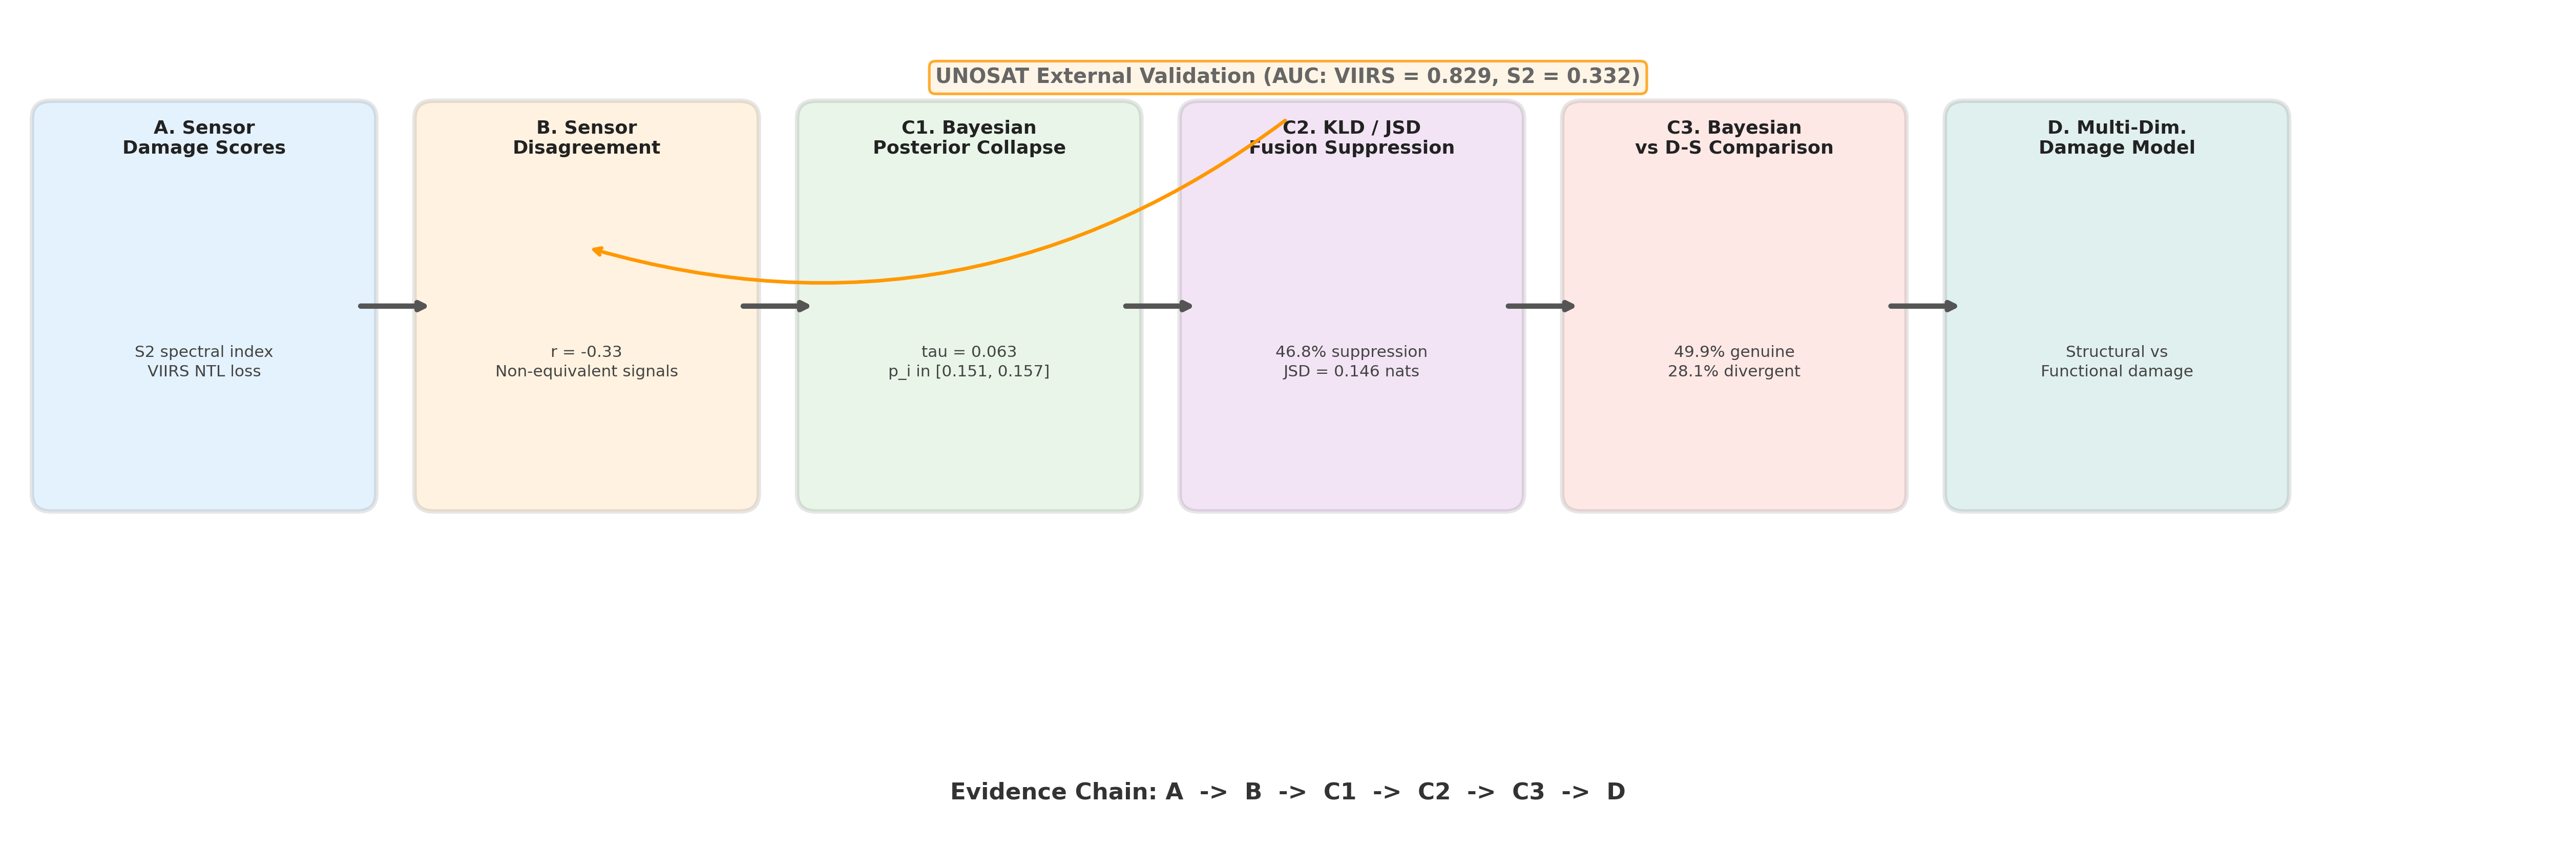
\includegraphics[width=0.98\textwidth]{figures/fig1_workflow_v4.png}
\caption{\textbf{Overall evidence-chain workflow.} The study proceeds
through six linked stages: (A) independent construction of S2 and VIIRS
damage scores; (B) identification of systematic sensor disagreement
($r=-0.33$); (C1) Bayesian hierarchical fusion revealing posterior collapse
under a single latent state ($\tau=0.063$); (C2) KLD/JSD quantification of
fusion suppression ($46.8\%$); (C3) comparison of Bayesian and
Dempster-Shafer fusion paradigms ($49.9\%$ genuine agreement, $28.1\%$
divergent); and (D) synthesis toward a multi-dimensional damage model.
UNOSAT external validation anchors stages B through C3 as a reference
benchmark.}
\label{fig:workflow}
\end{center}
\end{figure}

The principal contributions are: (1)~a Bayesian hierarchical uncertainty
framework for fusing S2 and VIIRS damage probabilities without requiring
ground-truth labels; (2)~a quantitative decomposition of single-sensor
information, fused information, and inter-sensor conflict using KLD and
JSD; and (3)~a grid-level comparison of Bayesian point-estimate fusion with
D-S interval-based evidence combination under conflicting evidence.
Figure~\ref{fig:workflow} illustrates the overall evidence chain.

% =====================================================================
\section{Related Work}\label{sec:related}

\subsection{Remote Sensing for Damage Assessment}

Satellite-based damage assessment has advanced substantially with the
availability of high-resolution optical imagery and synthetic aperture
radar (SAR). Pre- and post-event change detection using spectral indices,
texture features, and machine learning classifiers has been applied to
earthquakes, hurricanes, and armed conflicts \cite{lebedev2022}. The
UNOSAT program provides operational damage assessments through visual
interpretation of very-high-resolution imagery, producing building-level
damage classifications that serve as external reference labels for
validation \cite{unosat2022}. However, optical methods are limited by cloud
cover and primarily detect structural damage visible from above; functional
damage such as power loss or economic disruption requires complementary
data sources.

\subsection{Nighttime Lights and Functional Disruption}

Nighttime light (NTL) remote sensing has emerged as a valuable tool for
detecting human activity disruption during conflicts and disasters. The
VIIRS DNB sensor, with its improved radiometric calibration and higher
spatial resolution compared to legacy DMSP-OLS, enables detection of
sub-city-scale changes in illumination. Studies of the Syria conflict
\cite{li2018}, the Yemen civil war, and the 2022 Russia-Ukraine conflict
\cite{xiao2024} have demonstrated that NTL reductions correlate with
conflict intensity and population displacement. The NASA Black Marble
product suite (VNP46) provides cloud-free, atmospheric-corrected NTL
composites that have been validated for disaster damage detection across
hurricanes, earthquakes, and tornadoes \cite{zhang2023}. A key limitation
is that NTL loss conflates multiple processes---building destruction, power
grid damage, and evacuation---so it cannot independently distinguish
structural from functional damage.

\subsection{Bayesian Hierarchical Fusion}

Bayesian hierarchical models provide a principled framework for combining
multiple data sources while propagating uncertainty through all levels of
the model. In the context of multi-sensor fusion, hierarchical structures
allow sensor-specific biases and noise levels to be estimated from the
data, and missing observations are handled naturally through the
hierarchical structure \cite{gelman2006}. The No-U-Turn Sampler (NUTS)
\cite{hoffman2014} enables efficient MCMC inference for models with
hundreds to thousands of parameters. A critical but often implicit
assumption in such models is that all sensors provide noisy observations of
a shared latent quantity. When this assumption is violated---as when
sensors measure physically distinct phenomena---the model may exhibit
extreme shrinkage and loss of spatial resolution, a phenomenon we
characterize quantitatively through the KLD/JSD framework.

\subsection{Dempster-Shafer Evidence Theory}

Dempster-Shafer (D-S) theory \cite{dempster1967,shafer1976} provides an
alternative to Bayesian probability for reasoning under uncertainty. Unlike
Bayesian approaches that require a single probability distribution over
mutually exclusive hypotheses, D-S assigns belief masses to subsets of the
hypothesis space, allowing explicit representation of ignorance. When
evidence from multiple sources is combined via Dempster's rule, conflict
between sources is quantified by the conflict coefficient $K$. D-S has been
applied to multi-sensor remote sensing fusion, land-cover classification,
and damage assessment, where it preserves evidence conflict rather than
forcing resolution into a single probability \cite{lebedev2022}.

\subsection{Information-Theoretic Divergence for Sensor Comparison}

Kullback-Leibler (KL) divergence \cite{kullback1951} and Jensen-Shannon
divergence (JSD) \cite{lin1991} provide information-theoretic tools for
comparing probability distributions. In multi-sensor contexts, KL
divergence can quantify how much information each sensor contributes
relative to a reference distribution, while the symmetric JSD measures the
dissimilarity between two sensor-specific posteriors. Recent work has
applied these tools to model comparison and sensor selection in remote
sensing, but their application to quantifying \emph{fusion suppression}---the
extent to which combining conflicting sensors reduces usable
information---has received limited attention. This study contributes a
computationally tractable Bernoulli-level KLD/JSD framework that decomposes
total information into single-sensor gain, spatial differentiation, and
fusion suppression components.

% =====================================================================
\section{Study Area and Data}\label{sec:data}

\subsection{Mariupol Area of Interest}

The study area covers Mariupol and surroundings in southeastern Ukraine
(37.42\textdegree{}E--37.72\textdegree{}E, 47.05\textdegree{}N--47.18\textdegree{}N),
a region that experienced extensive structural and functional damage during
the 2022 conflict. The AOI spans approximately 23~km east-west by 14~km
north-south and is divided into 1{,}380 grid cells at 500~m resolution.

\subsection{Sentinel-2 Imagery}

Sentinel-2 Level-2A surface reflectance products were acquired for
pre-event (2021-05-23) and post-event (2022-05-08) dates, covering tiles
T37TCN and T37TDN. The pre-event date was chosen to match the same
phenological period one year prior. Spectral indices (NDVI, NBR, and
soil-adjusted variants) were computed from 10~m and 20~m bands, and per-index
deltas were normalized by pre-event spatial standard deviations. The S2
damage score $p_{\text{S2}}$ was obtained by averaging z-scores and
transforming to $[0,1]$ via the logistic function.

\subsection{VIIRS Nighttime Light Data}

VIIRS DNB monthly composite data (VNP46A3) were obtained for matching pre-
and post-event periods. DNB radiance values were filtered using the
mandatory quality flag. Per-grid mean NTL radiance and the relative NTL
loss rate $R_i = (L_{\text{pre},i} - L_{\text{post},i})/L_{\text{pre},i}$
were computed at 500~m resolution and transformed to $p_{\text{VIIRS}}$ via
sigmoid calibration.

\subsection{UNOSAT External Reference Labels}

UNOSAT damage assessment data for the Livoberezhnyi District of Mariupol
(dated 12 May 2022), produced through visual interpretation of
very-high-resolution satellite imagery, were used as an external reference.
Building footprints were spatially joined to the 500~m grid. A strict
matching protocol treated Main\_Dam\_1~$=14$ (destroyed) as positive and
Main\_Dam\_1~$=6$ (no visible damage) as negative, yielding 995 labeled
grids (32.8\% positive). UNOSAT is an external reference rather than
absolute ground truth; it captures visually identifiable structural damage
but may miss functional damage or sub-detection-threshold alteration.

\begin{table}[htp]
\centering
\caption{Data sources and preprocessing summary.}
\label{tab:data}
\begin{tabular}{@{}lllll@{}}
\toprule
\textbf{Source} & \textbf{Product} & \textbf{Pre-Date} & \textbf{Post-Date} & \textbf{Resolution} \\
\midrule
Sentinel-2 MSI  & L2A Surface Reflectance  & 2021-05-23 & 2022-05-08 & 10--20~m (500~m grid) \\
VIIRS DNB       & VNP46A3 Monthly Composite & 2021-05    & 2022-05    & 500~m native \\
UNOSAT          & Visual Damage Assessment  & ---        & 2022-05-12 & Building-level \\
\midrule
\textbf{Grid}   & \textbf{Cells} & \textbf{CRS} & \textbf{Valid S2} & \textbf{Valid VIIRS} \\
500~m fishnet   & 1{,}380        & WGS84        & 1{,}131 (82.0\%)   & 1{,}268 (91.9\%) \\
\bottomrule
\end{tabular}
\end{table}

% =====================================================================
\section{Methods}\label{sec:methods}

\subsection{Sentinel-2 Spectral Damage Index}

For each 500~m grid cell, spectral indices are computed from all valid
10~m and 20~m pixels within the cell for both pre- and post-event images.
The per-index change $\Delta_k$ is normalized by the pre-event spatial
standard deviation $\sigma_k$ to produce a z-score. The S2 damage
probability is the logistic transform of the mean z-score, clipped to
$[10^{-4}, 1-10^{-4}]$.

\subsection{VIIRS Nightlight-Loss Index}

The VIIRS damage probability $p_{\text{VIIRS},i}$ is derived from the
relative NTL loss rate. Negative loss rates are clamped to zero, and the
loss rate is transformed via sigmoid calibration on the empirical
distribution. Grids with $<10$ valid DNB observations in either period are
marked as missing.

\subsection{UNOSAT External Validation}

Each damage score is evaluated as a binary classifier against the UNOSAT
strict label set. Metrics include AUC, PR-AUC, Brier score, and Spearman
rank correlation. Validation is performed for S2, VIIRS, logit-averaged
fusion, and D-S belief, plausibility, and midpoint.

\subsection{Bayesian Hierarchical Uncertainty Fusion}\label{sec:bayes}

We specify a three-level logit-normal hierarchical model with a single
latent damage state. Let $y_{ik} = \text{logit}(p_{ik})$ for sensor
$k \in \{\text{S2}, \text{VIIRS}\}$ at grid $i$:

\begin{align}
\text{Level 1:}\quad
  y_{i,\text{S2}} &\sim \mathcal{N}(\theta_i + \delta_{\text{S2}},\;
                     \sigma_{\text{S2}}^2) \label{eq:L1s2}\\
  y_{i,\text{VIIRS}} &\sim \mathcal{N}(\theta_i,\;
                         \sigma_{\text{VIIRS}}^2) \label{eq:L1v}\\
\text{Level 2:}\quad
  \theta_i &= \text{logit}(p_i) = \mu + \eta_i,\quad
  \eta_i \sim \mathcal{N}(0, \tau^2) \label{eq:L2}\\
\text{Level 3:}\quad
  \mu &\sim \mathcal{N}(0, 2^2),\quad
  \tau \sim \text{HalfCauchy}(1),\quad
  \sigma_k \sim \text{HalfCauchy}(0.5) \label{eq:L3}
\end{align}

The bias $\delta_{\text{S2}}$ captures S2's systematic offset. Posterior
inference uses NUTS with 4 chains of 1{,}000 tuning and 1{,}000 sampling
iterations. Single-sensor baselines are fitted by omitting the unused
sensor's likelihood.

\subsection{KLD/JSD Information Gain Analysis}\label{sec:kld}

We quantify information using Bernoulli-level KL divergence. For two
Bernoulli distributions parameterized by $p$ and $q$:

\begin{equation}
\mathrm{KL}(p \,\|\, q) = p\log\frac{p}{q} + (1-p)\log\frac{1-p}{1-q}
\label{eq:kl}
\end{equation}

\begin{equation}
\mathrm{JSD}(p, q) = \tfrac{1}{2}\mathrm{KL}(p \,\|\, m)
  + \tfrac{1}{2}\mathrm{KL}(q \,\|\, m),\quad
  m = \tfrac{1}{2}(p+q)
\label{eq:jsd}
\end{equation}

All divergences use natural logarithms (nats). We compute: (1)~single-sensor
gain against neutral prior $p=0.5$; (2)~spatial differentiation against
each model's global mean; (3)~fusion suppression,
$\text{suppression} = (\max\text{KL} - \text{KL}_{\text{both}}) /
\max\text{KL}$, measuring the fraction of best single-sensor information
lost in fusion.

\subsection{Dempster-Shafer Evidence Fusion and Consistency
Comparison}\label{sec:ds}

BPAs are constructed for states Damage ($D$), No Damage ($N$), and
Uncertainty ($U$): $m_k(D) = \alpha_k p_k$, $m_k(N) = \alpha_k (1-p_k)$,
$m_k(U)=1-\alpha_k$, where $\alpha_k$ reflects sensor reliability.
Dempster's rule yields $\text{Bel}(D) = m_{12}(D)/(1-K)$ and
$\text{Pl}(D) = (m_{12}(D)+m_{12}(U))/(1-K)$. Consistency classification
uses: \emph{genuine agreement} (Bayesian mean within narrow D-S interval),
\emph{uncertainty-compatible} (mean within wide interval),
\emph{weak consistent} (CI overlap), and \emph{divergent} (CI disjoint).

% =====================================================================
\section{Results}\label{sec:results}

\subsection{S2 and VIIRS Provide Non-Equivalent Damage Signals}\label{sec:res-disagree}

\begin{figure}[htp]
\begin{center}
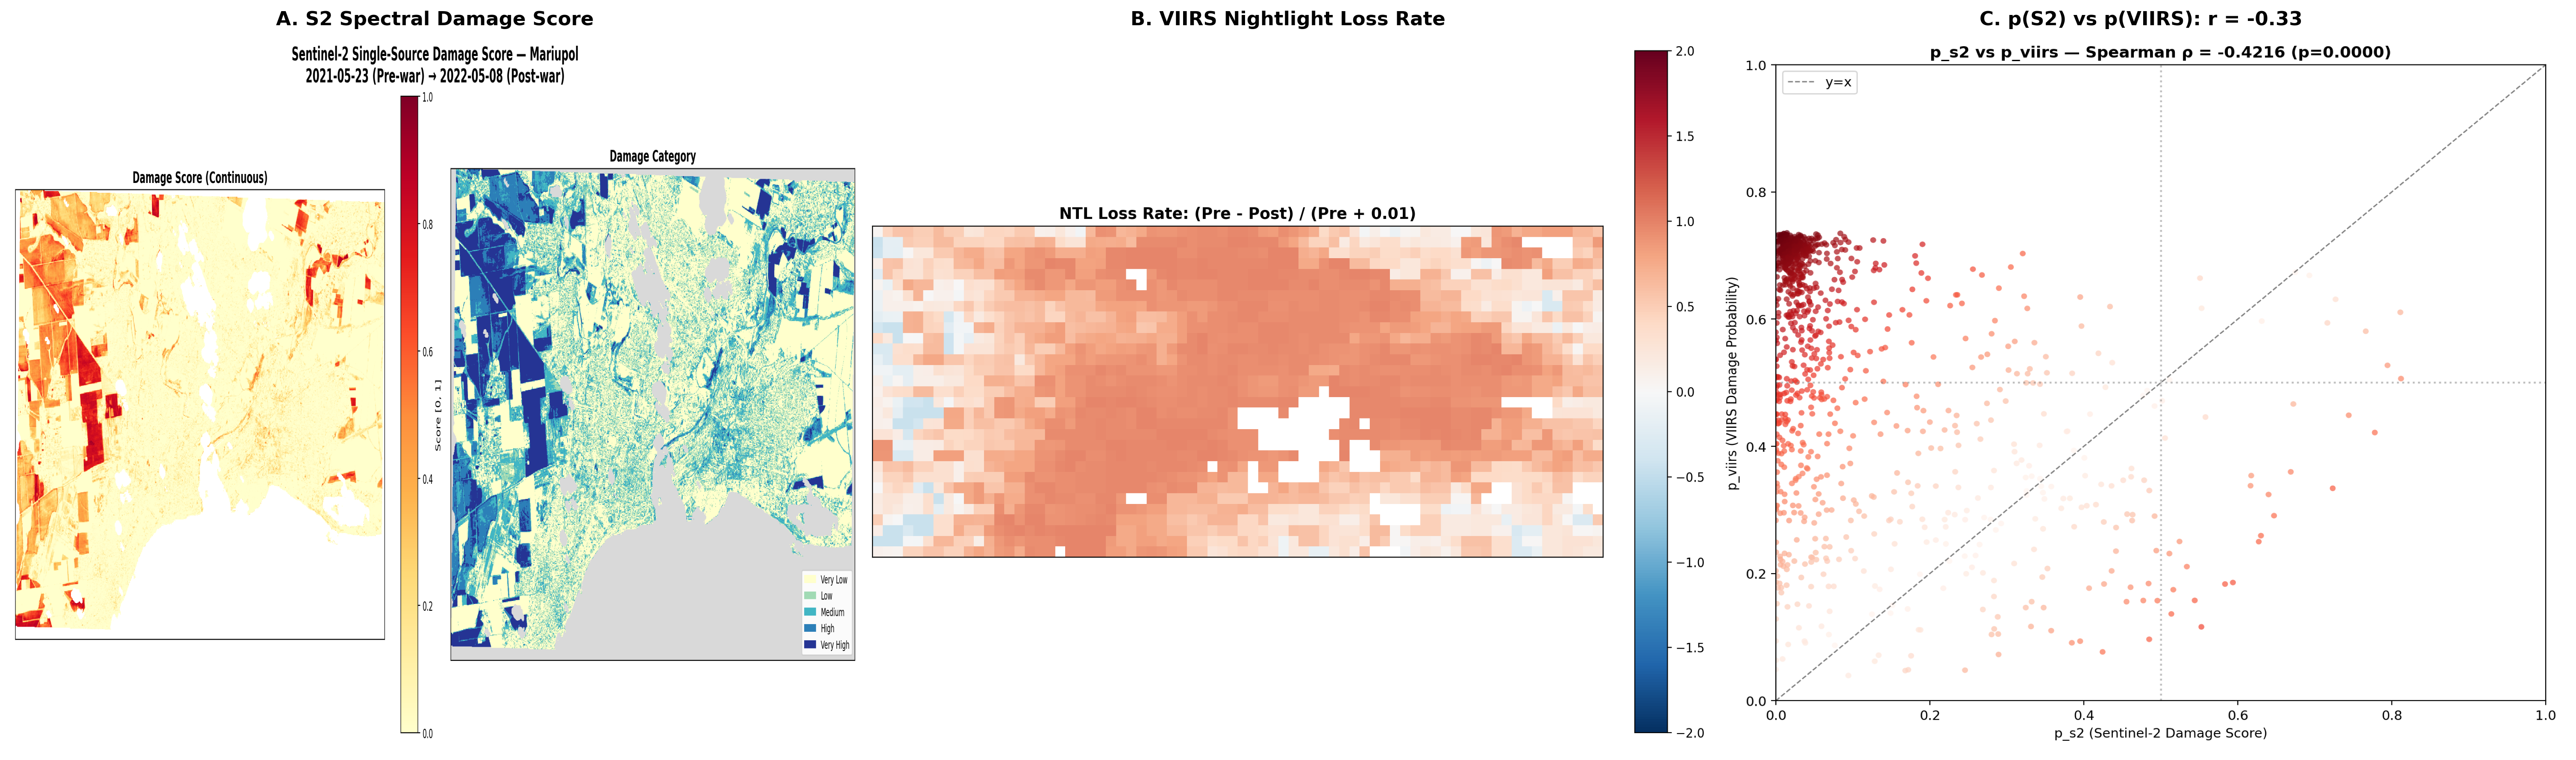
\includegraphics[width=0.95\textwidth]{figures/fig2_sensor_disagreement_v4.png}
\caption{\textbf{S2 and VIIRS capture distinct damage dimensions.}
(A)~S2 spectral damage score highlights urban-core surface alteration.
(B)~VIIRS NTL loss rate shows a more diffuse spatial pattern extending into
peri-urban areas. (C)~The scatter plot reveals a negative correlation
($r = -0.33$) between the two scores: grids with high S2 damage do not
systematically correspond to grids with high VIIRS damage. This indicates
that S2 and VIIRS are not redundant observations of a single latent damage
state.}
\label{fig:disagree}
\end{center}
\end{figure}

Figure~\ref{fig:disagree} establishes the foundational observation. The S2
score (Panel~A) concentrates elevated values in the urban core and
industrial zones, consistent with spectral signatures of exposed rubble and
altered vegetation. The VIIRS NTL loss (Panel~B) shows a more diffuse
pattern extending into peri-urban areas, consistent with widespread power
outages and population displacement beyond the footprint of structural
destruction. The scatter plot (Panel~C) quantifies the disagreement:
Pearson $r = -0.33$. Grids form two distinct clusters---S2-high/VIIRS-low
(structural damage with retained nightlight) and S2-low/VIIRS-high
(functional loss without visible structural change). These are genuine
physical phenomena, not measurement errors.

\subsection{UNOSAT Validation Under This Reference Setting}\label{sec:res-unosat}

\begin{figure}[htp]
\begin{center}
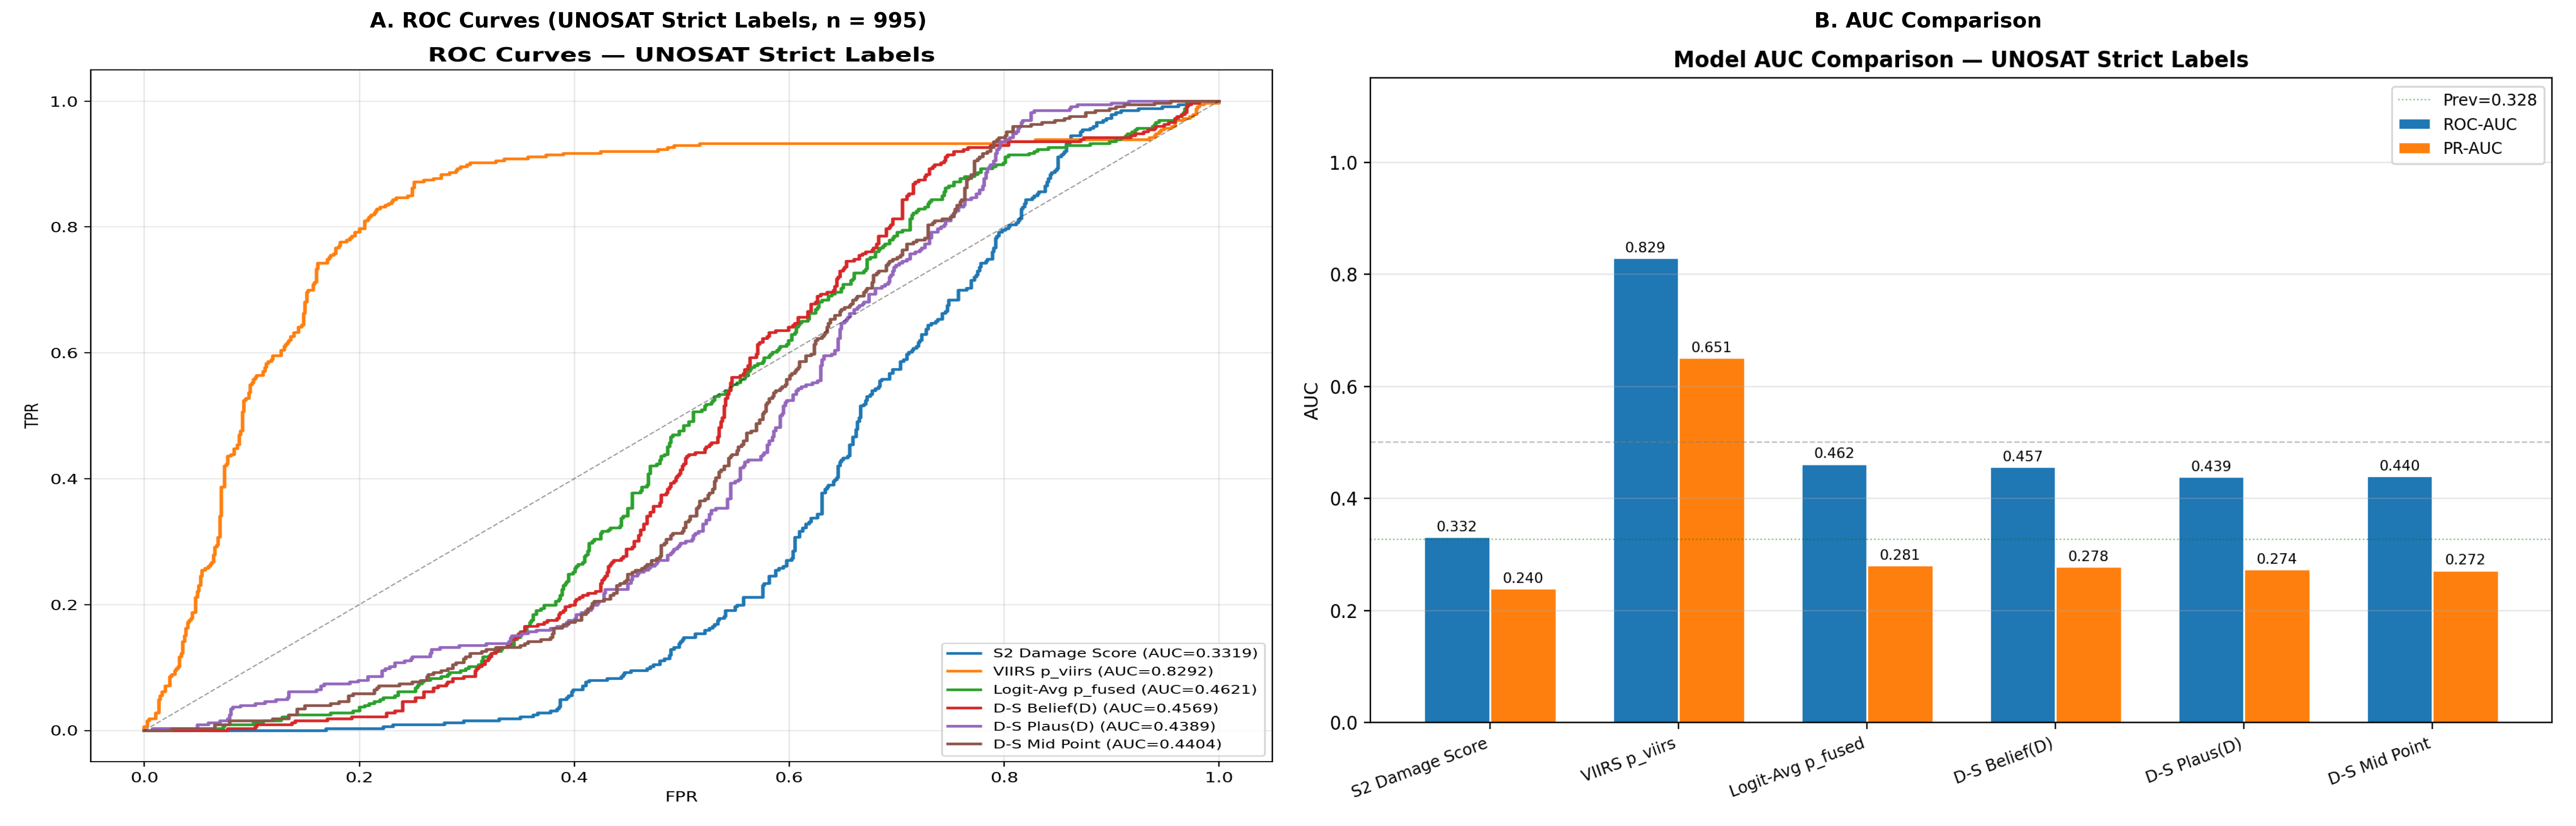
\includegraphics[width=0.95\textwidth]{figures/fig3_unosat_validation_v4.png}
\caption{\textbf{UNOSAT external validation.}
(A)~ROC curves against UNOSAT strict labels ($n=995$, $32.8\%$ positive).
VIIRS shows stronger agreement with UNOSAT under this validation setting
(AUC~$=0.829$, Spearman $r=0.535$). The current S2-derived index is weakly
aligned (AUC~$=0.332$, below the random baseline). All fusion-based scores
perform below VIIRS alone: logit-average (AUC~$=0.462$), D-S belief
(AUC~$=0.457$), plausibility (AUC~$=0.439$), and midpoint (AUC~$=0.440$).
(B)~AUC barplot comparison confirms that adding S2 degrades discriminative
performance under every aggregation method tested.}
\label{fig:unosat}
\end{center}
\end{figure}

Figure~\ref{fig:unosat} presents external validation. VIIRS shows stronger
agreement with UNOSAT reference labels (AUC~$=0.829$, Spearman $r=0.535$,
Brier~$=0.222$), while the current S2-derived index is weakly aligned
(AUC~$=0.332$, $r=-0.274$, Brier~$=0.343$). All fusion-based
scores---logit-average (AUC~$=0.462$), D-S belief (AUC~$=0.457$),
plausibility (AUC~$=0.439$), midpoint (AUC~$=0.440$)---perform below VIIRS
alone, consistent with the hypothesis that combining a weakly aligned
signal with a well-aligned one introduces noise rather than complementary
information. The maximum F1 of $0.630$ (VIIRS) reflects the fact that
UNOSAT labels a specific subset of damage types. PR curves are provided in
Appendix~\ref{apd:pr}.

\subsection{Bayesian Hierarchical Fusion Collapses Under the Single Latent
State Assumption}\label{sec:res-bayes}

\begin{table}[htp]
\centering
\caption{Bayesian hyperparameter posterior estimates. All parameters
converged ($\hat{R} < 1.01$, 1 divergence in 4{,}000 draws).}
\label{tab:bayes_params}
\begin{tabular}{@{}lrrrrr@{}}
\toprule
\textbf{Parameter} & \textbf{Mean} & \textbf{SD} & \textbf{2.5\%} & \textbf{97.5\%} & \textbf{$\hat{R}$} \\
\midrule
$\mu$ (population mean, logit)        & $-1.695$ & $0.042$ & $-1.781$ & $-1.613$ & $1.000$ \\
$\tau$ (between-grid heterogeneity)   & $ 0.063$ & $0.047$ & $ 0.004$ & $ 0.172$ & $1.000$ \\
$\sigma_{\text{S2}}$ (S2 noise)       & $ 2.685$ & $0.059$ & $ 2.575$ & $ 2.803$ & $1.000$ \\
$\sigma_{\text{VIIRS}}$ (VIIRS noise) & $ 0.904$ & $0.018$ & $ 0.869$ & $ 0.940$ & $1.000$ \\
$\delta_{\text{S2}}$ (S2 bias)        & $-1.705$ & $0.042$ & $-1.789$ & $-1.624$ & $1.000$ \\
\bottomrule
\end{tabular}
\end{table}

\begin{figure}[htp]
\begin{center}
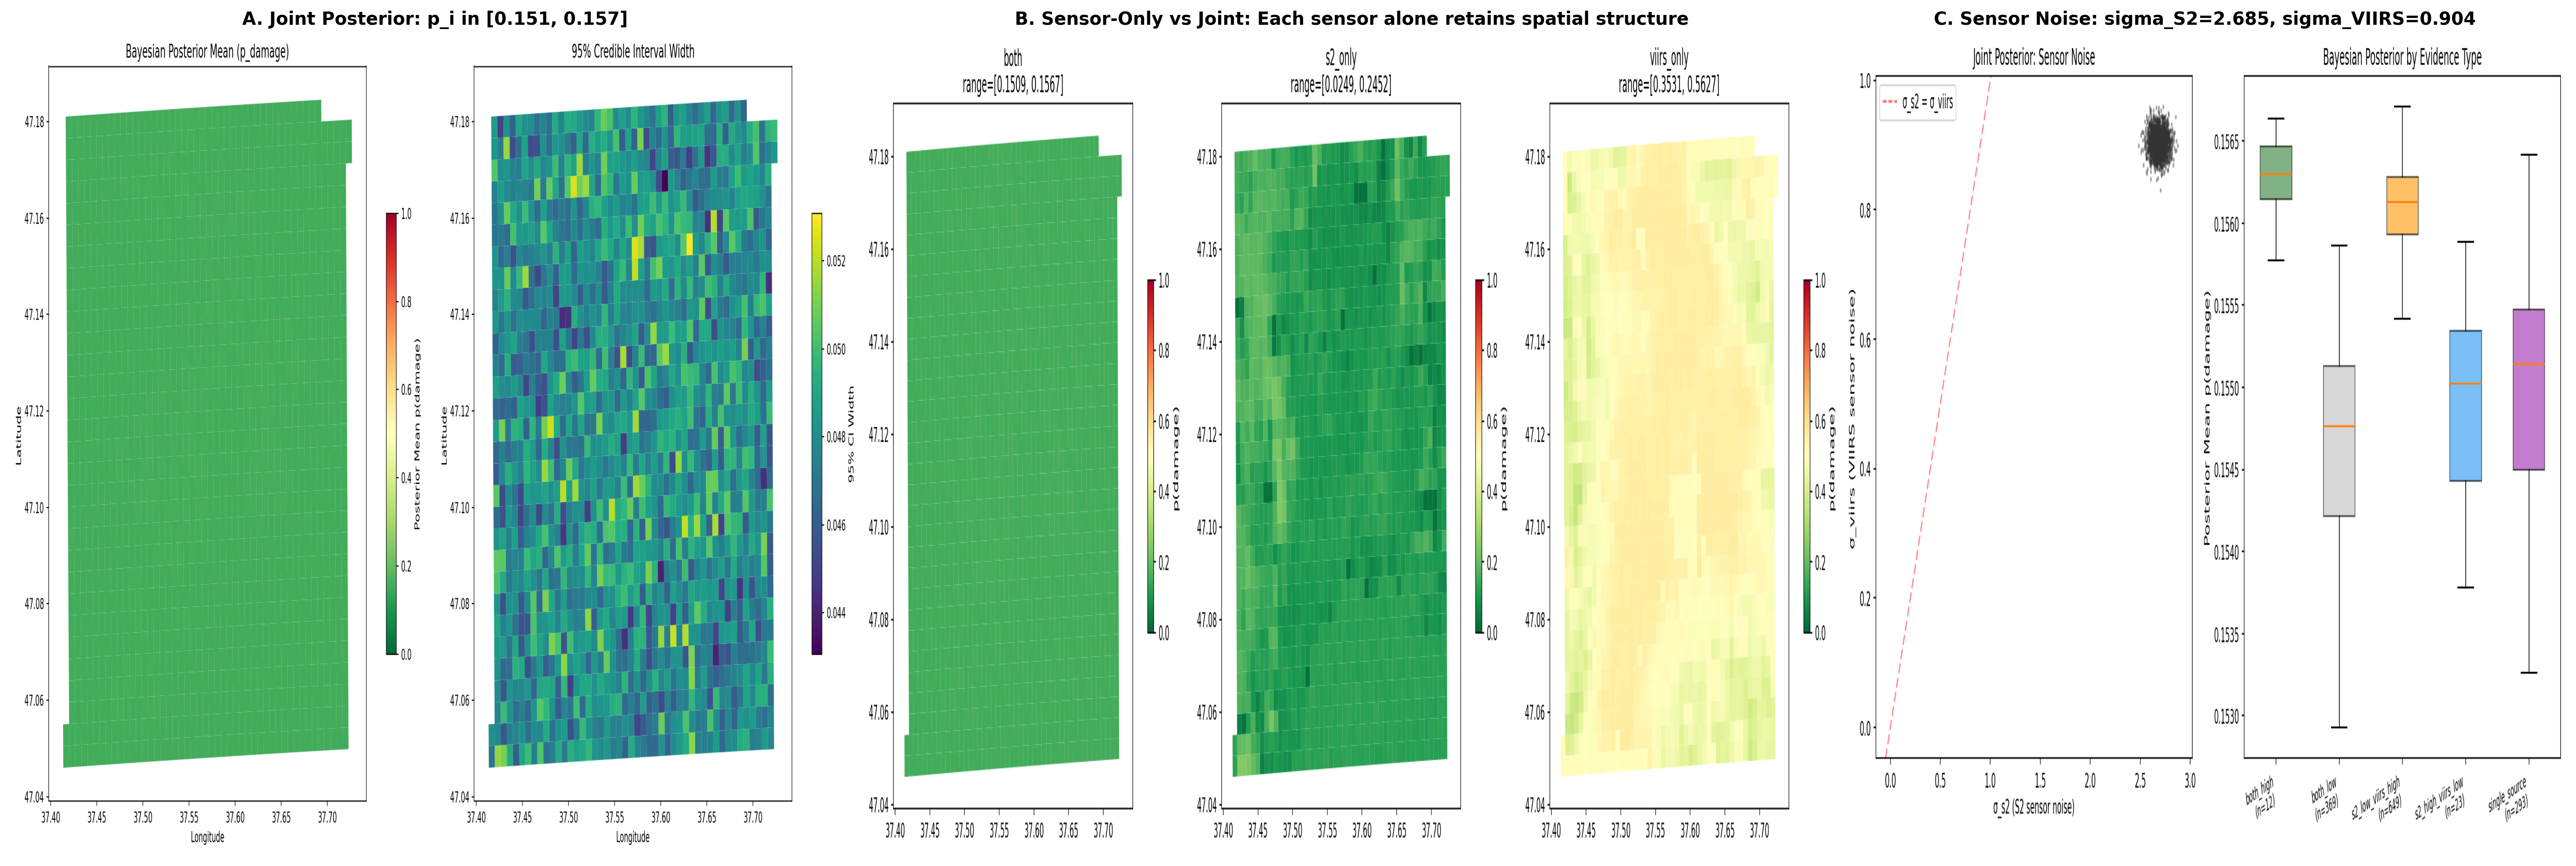
\includegraphics[width=0.95\textwidth]{figures/fig4_bayesian_collapse_v4.png}
\caption{\textbf{Bayesian posterior collapse under single latent state
assumption.}
(A)~Joint posterior mean map: $p_i \in [0.151, 0.157]$, spatially
near-uniform. (B)~Sensor-only comparison: S2-only spans $[0.025, 0.245]$
(22 pp range); VIIRS-only spans $[0.353, 0.563]$ (21 pp range); the joint
model collapses both into a 0.006 pp band. (C)~Sensor noise estimates:
$\sigma_{\text{S2}} = 2.685$, approximately $3\times$ larger than
$\sigma_{\text{VIIRS}} = 0.904$ on the logit scale.}
\label{fig:bayes}
\end{center}
\end{figure}

Table~\ref{tab:bayes_params} and Figure~\ref{fig:bayes} present the
Bayesian results. Three estimates jointly explain the collapse. First,
$\tau = 0.063$ (95\% CI: $[0.004, 0.172]$) indicates essentially no shared
grid-level heterogeneity after accounting for sensor bias and noise.
Second, $\sigma_{\text{S2}} = 2.685$ is $\sim3\times$ $\sigma_{\text{VIIRS}}
= 0.904$; the model learns S2 is less precise. Third, $\delta_{\text{S2}} =
-1.705$ captures S2's systematic lower reporting. Figure~\ref{fig:bayes}A:
the joint posterior is near-uniform---this map cannot distinguish a
destroyed city block from an intact field. Figure~\ref{fig:bayes}B: each
single-sensor model retains spatial structure (21--22 pp ranges); collapse
occurs only under joint fusion. Single-sensor MCMC diagnostics were weaker
(S2-only: 263 divergences, $\hat{R}_{\max}=1.21$; VIIRS-only: 122
divergences, $\hat{R}_{\max}=1.35$), so single-sensor ranges are diagnostic
comparisons (see Limitations).

\subsection{KLD/JSD Shows Information Conflict Rather Than Information
Absence}\label{sec:res-kld}

\begin{table}[htp]
\centering
\caption{KLD/JSD information gain summary. All metrics in nats, computed
at the Bernoulli probability level with neutral prior $p=0.5$.}
\label{tab:kld}
\begin{tabular}{@{}lrrrr@{}}
\toprule
\textbf{Metric} & \textbf{Mean} & \textbf{Median} & \textbf{Min} & \textbf{Max} \\
\midrule
KL(S2 $\|$ neutral)          & 0.496 & 0.501 & 0.301 & 0.591 \\
KL(VIIRS $\|$ neutral)       & 0.007 & 0.006 & 0.000 & 0.072 \\
KL(Both $\|$ neutral)        & 0.261 & 0.261 & 0.259 & 0.269 \\
KL(S2 $\|$ S2$_{\text{global}}$)    & 0.003 & 0.001 & 0.000 & 0.050 \\
KL(VIIRS $\|$ VIIRS$_{\text{global}}$) & 0.007 & 0.005 & 0.000 & 0.075 \\
$\mathbf{KL(Both \| Both_{\text{global}})}$ & $\mathbf{\approx 0}$ & $\mathbf{\approx 0}$ & $\mathbf{\approx 0}$ & $\mathbf{<0.001}$ \\
JSD(S2, VIIRS)               & 0.146 & 0.150 & 0.053 & 0.212 \\
Fusion KL loss               & 0.235 & 0.240 & 0.041 & 0.329 \\
Fusion suppression ratio     & 0.468 & 0.479 & 0.137 & 0.557 \\
\bottomrule
\end{tabular}
\end{table}

\begin{figure}[htp]
\begin{center}
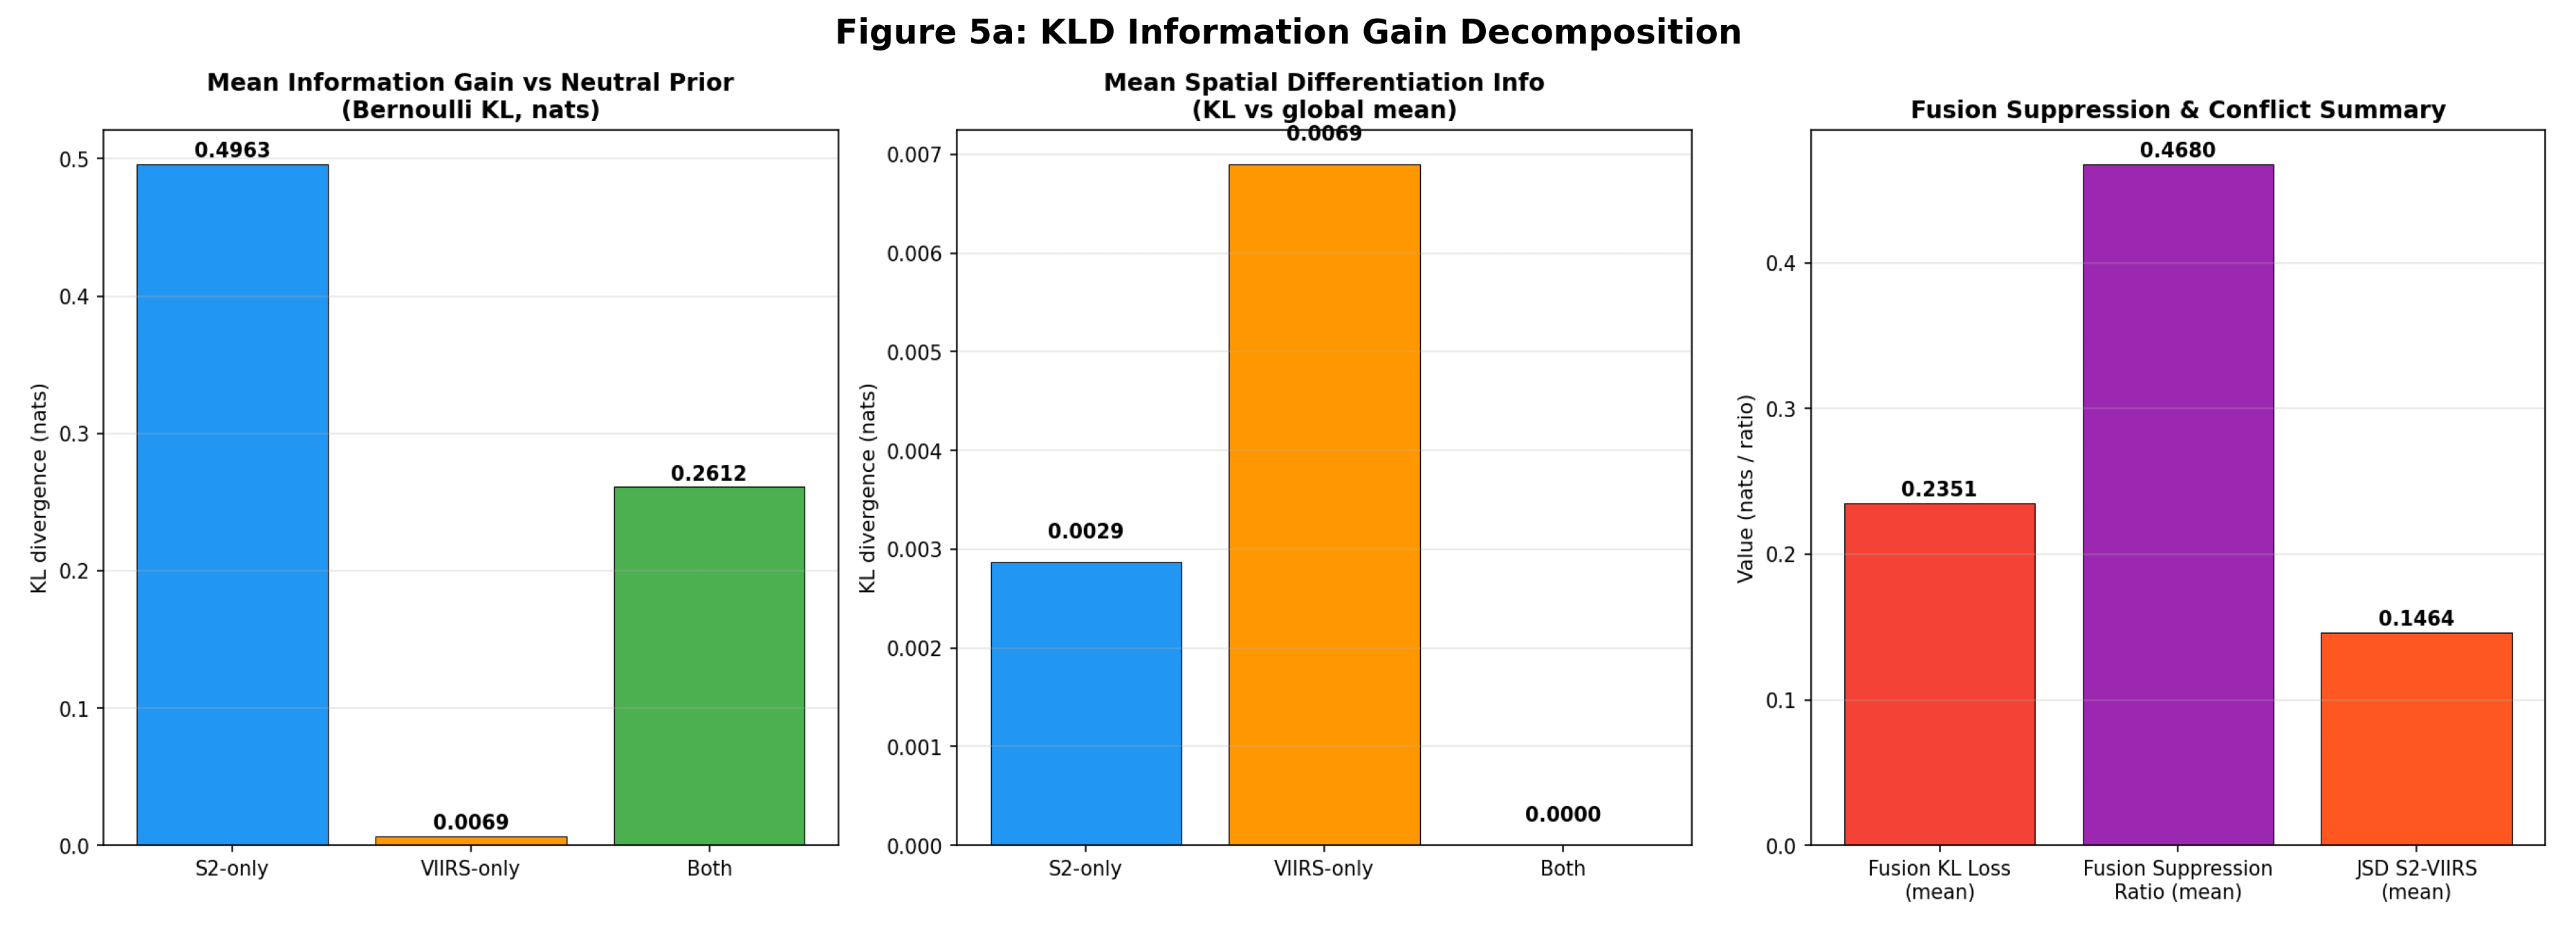
\includegraphics[width=0.95\textwidth]{figures/fig5a_kld_summary_v4.png}
\caption{\textbf{KLD information gain decomposition.} S2 deviates strongly
from neutral prior ($p=0.05$ vs.\ $p=0.5$, KL~$=0.496$ nats); VIIRS remains
near neutral (KL~$=0.007$ nats). Spatial differentiation (KL vs.\ global
mean, gray bars) is near zero for the fused model---three orders of
magnitude below single-sensor values.}
\label{fig:kld_summary}
\end{center}
\end{figure}

\begin{figure}[htp]
\begin{center}
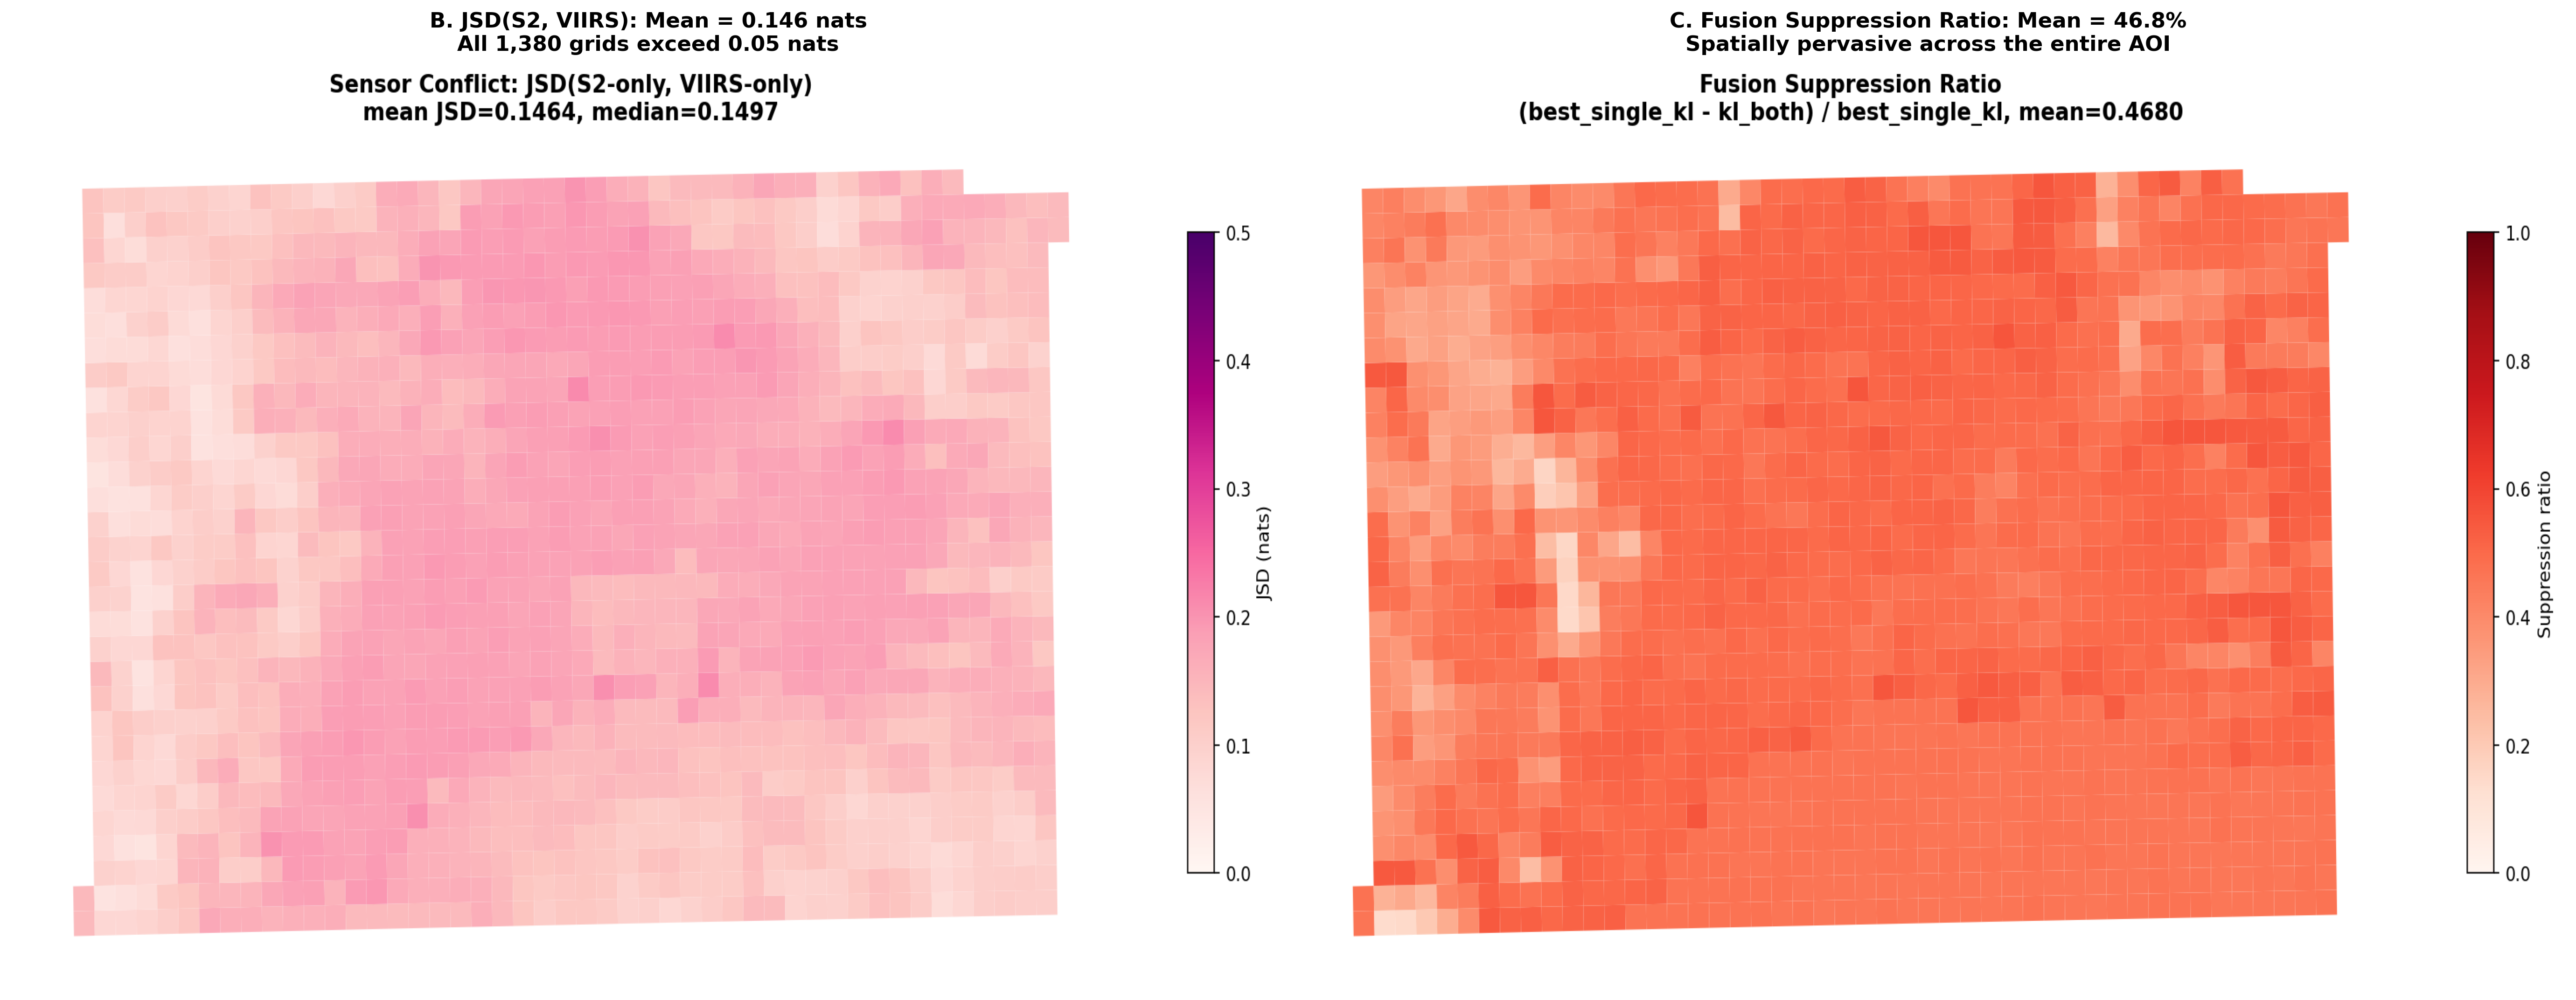
\includegraphics[width=0.95\textwidth]{figures/fig5b_kld_maps_v4.png}
\caption{\textbf{Spatial conflict and fusion suppression maps.}
(B)~JSD(S2, VIIRS): every grid exceeds $0.05$ nats (mean $0.146$, range
$[0.053, 0.212]$). Conflict is highest in the urban core and industrial
periphery. (C)~Fusion suppression ratio: mean $46.8\%$ (median $47.9\%$),
spatially pervasive---this is an AOI-wide phenomenon, not confined to a few
outlier grids.}
\label{fig:kld_maps}
\end{center}
\end{figure}

Table~\ref{tab:kld} and Figures~\ref{fig:kld_summary}--\ref{fig:kld_maps}
present the KLD/JSD decomposition. The barplot (Figure~\ref{fig:kld_summary})
reveals an asymmetry: KL(S2 $\|$ neutral)~$=0.496$ nats because S2 is
concentrated near $p\approx0.05$; KL(VIIRS $\|$ neutral)~$=0.007$ nats
because VIIRS is near $p\approx0.50$. KL vs.\ neutral measures deviation
from uncertainty, not accuracy. The critical diagnostic is spatial
differentiation: KL(S2 $\|$ S2$_{\text{global}}$)~$=0.003$ and KL(VIIRS
$\|$ VIIRS$_{\text{global}}$)~$=0.007$ nats, but KL(Both $\|$
Both$_{\text{global}}$) $\approx 0$ nats---spatial information is
eliminated under fusion.

Figure~\ref{fig:kld_maps}B shows that JSD(S2, VIIRS) exceeds $0.05$ nats
for every grid (mean $0.146$, max $0.212$). Conflict is systematic and
AOI-wide. The fusion suppression map (Figure~\ref{fig:kld_maps}C) averages
$46.8\%$ (range $[13.7\%, 55.7\%]$). The red-dominated map confirms this
is not driven by outliers. Conclusion: spatial information is not absent;
it is actively suppressed when conflicting evidence is forced into a single
latent state.

\subsection{Bayesian and D-S Behave Differently Under Conflicting
Evidence}\label{sec:res-ds}

\begin{table}[htp]
\centering
\caption{Bayesian vs.\ D-S consistency. Genuine agreement requires D-S
interval width below the 75th percentile ($0.184$).}
\label{tab:consistency}
\begin{tabular}{@{}lrrrr@{}}
\toprule
\textbf{Consistency Label} & \textbf{$N$} & \textbf{\%} &
  \textbf{Mean JSD} & \textbf{Mean D-S Width} \\
\midrule
Genuine agreement        & 689 & 49.9 & 0.153 & 0.197 \\
Uncertainty-compatible   & 141 & 10.2 & 0.166 & 0.277 \\
Weak consistent          & 128 &  9.3 & 0.148 & 0.216 \\
Divergent (low Bayes)    & 360 & 26.1 & 0.128 & 0.300 \\
Divergent (high Bayes)   &  28 &  2.0 & 0.124 & 0.093 \\
No D-S data              &  34 &  2.5 & ---   & ---   \\
\midrule
\textbf{Total}           & \textbf{1{,}380} & \textbf{100.0} & \textbf{0.146} & \textbf{0.225} \\
\bottomrule
\end{tabular}
\end{table}

\begin{figure}[htp]
\begin{center}
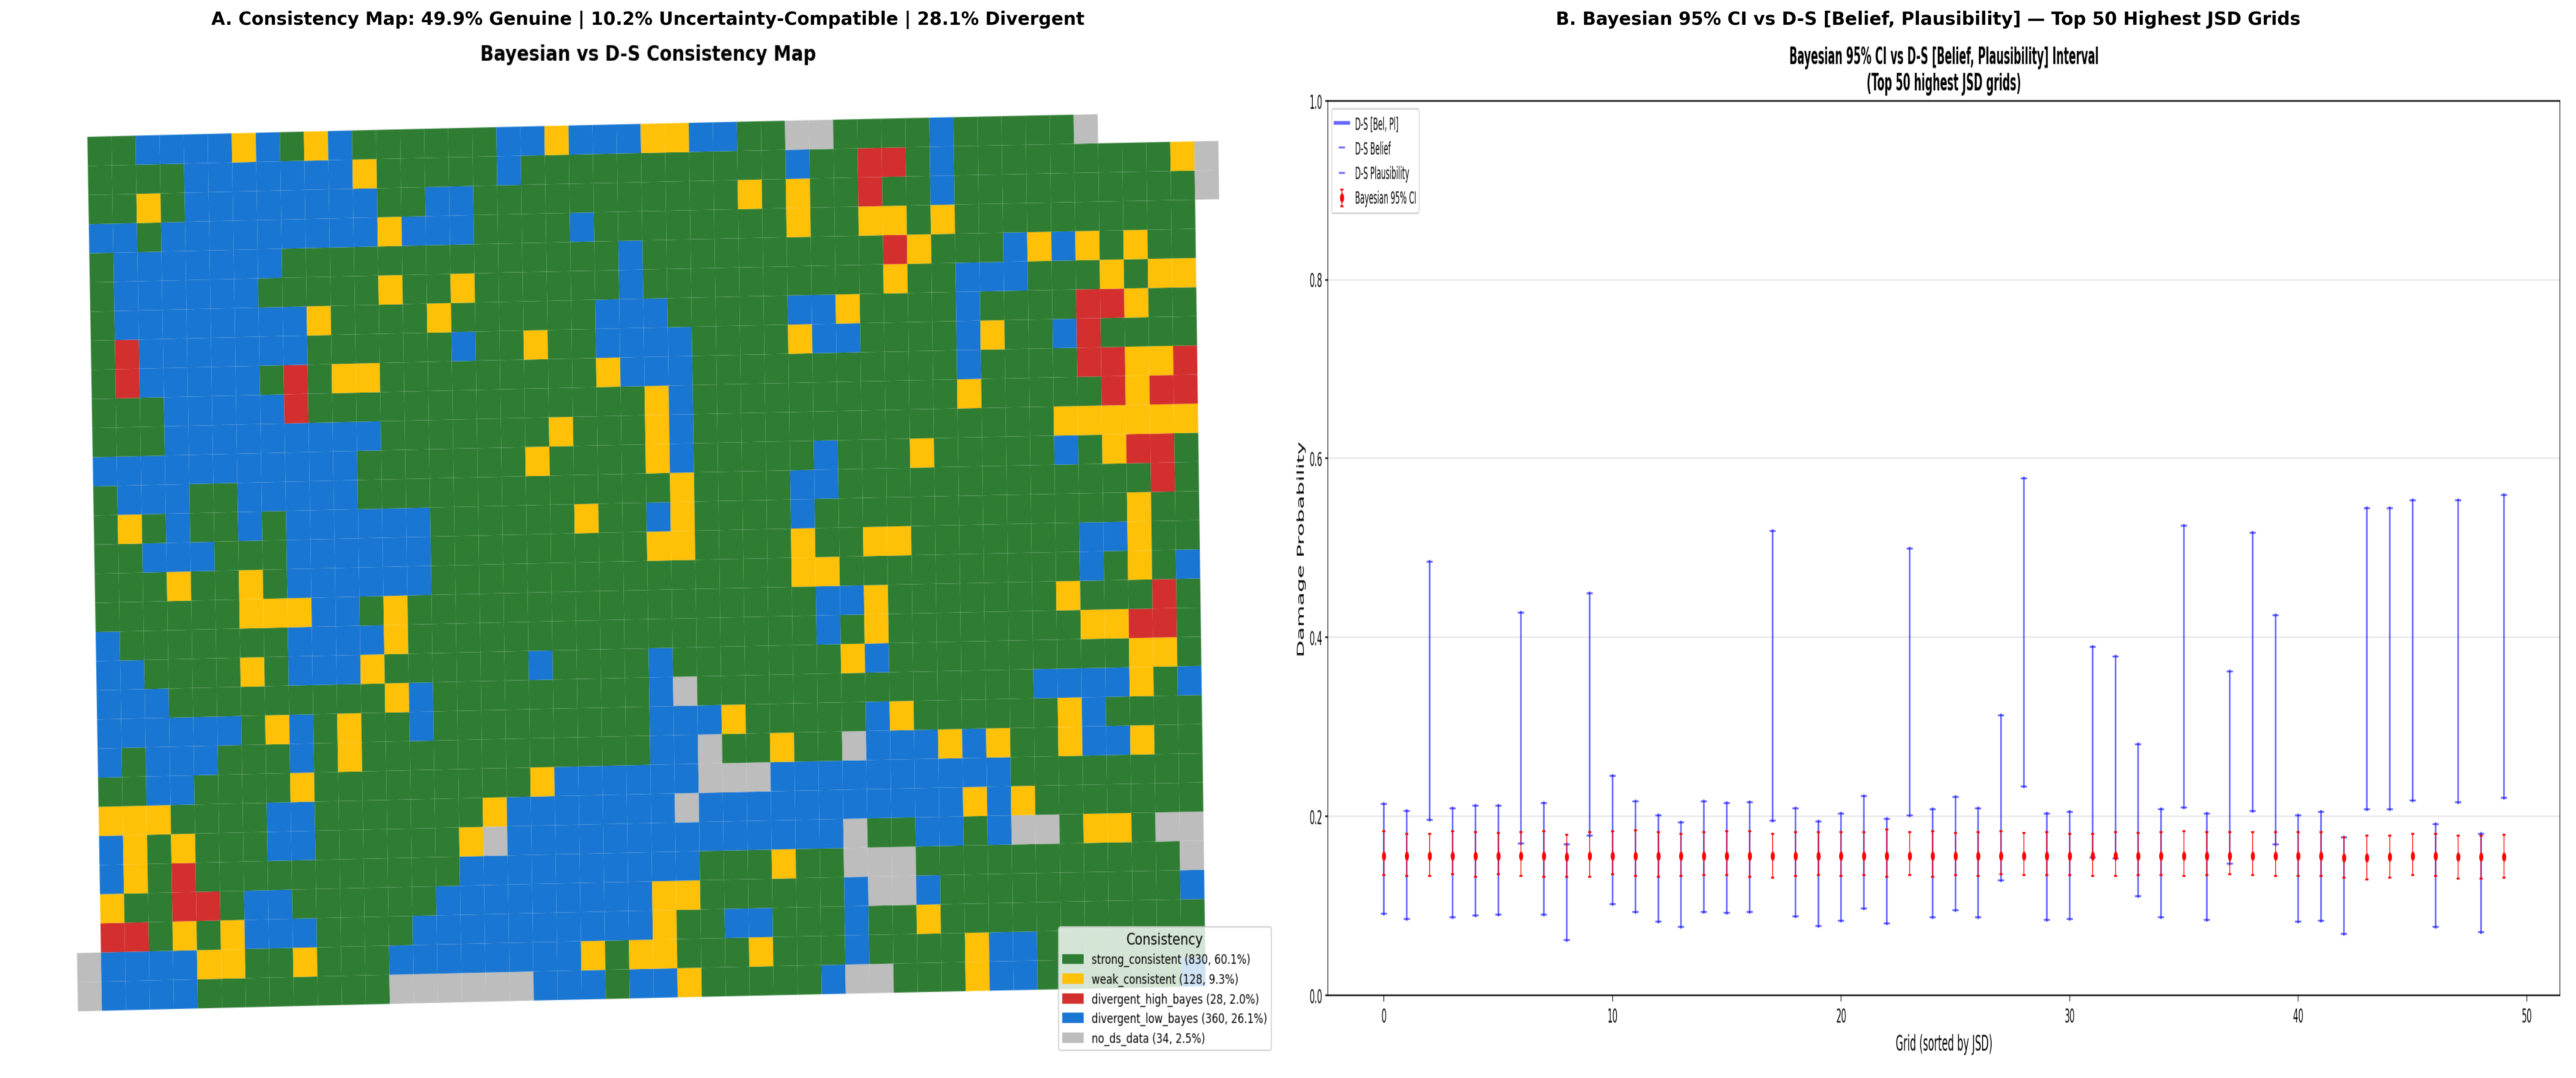
\includegraphics[width=0.95\textwidth]{figures/fig6_bayes_ds_v4.png}
\caption{\textbf{Bayesian vs.\ Dempster-Shafer under conflicting evidence.}
(A)~Consistency map: $49.9\%$ genuine agreement (green); $10.2\%$
uncertainty-compatible (yellow); $28.1\%$ divergent (red/blue). Divergence
concentrates in the urban core. (B)~Bayesian 95\% CI vs.\ D-S [Belief,
Plausibility] for the 50 highest-JSD grids. D-S intervals (blue) are
consistently wider than Bayesian CIs (red). The negative correlation
between JSD and Bayesian-DS distance ($r = -0.35$) indicates that the two
paradigms converge under high conflict (wide D-S intervals encompass the
Bayesian mean) and diverge under locally consistent but globally
conflicting evidence.}
\label{fig:ds}
\end{center}
\end{figure}

Table~\ref{tab:consistency} and Figure~\ref{fig:ds} provide the grid-level
comparison. $49.9\%$ of grids exhibit genuine agreement; $10.2\%$ are
uncertainty-compatible (wide D-S interval mechanically covers the Bayesian
mean). The largest divergent category is ``divergent\_low\_bayes''
($26.1\%$): Bayesian $p\approx0.155$ lies below D-S belief. In these
grids, D-S assigns high belief to damage (often from strong single-sensor
evidence), while Bayesian shrinkage pulls toward the population mean.
Approximately $60\%$ of these divergent grids are labeled undamaged by
UNOSAT, suggesting that the Bayesian shrinkage, while resulting in reduced
spatial resolution, is directionally consistent with the external reference
in a majority of these cases. The D-S intervals are consistently wider than
Bayesian CIs (mean width $0.225$ vs.\ $0.048$). JSD and Bayesian-DS
distance are negatively correlated ($r = -0.35$): high conflict widens D-S
intervals, which then more readily cover the Bayesian mean.

% =====================================================================
\section{Discussion}\label{sec:discussion}

\subsection{Sensor Conflict Is Not Sensor Failure}

The S2 and VIIRS damage indices disagree systematically because they
respond to different physical processes. S2 spectral change detects surface
alteration---exposed rubble, soil disturbance---that may or may not
indicate building destruction. VIIRS NTL loss detects reduced human
activity from structural damage, power failure, or displacement. These are
not measurement errors but genuine physical phenomena captured by different
sensing modalities. The JSD analysis confirms every grid exhibits
non-negligible conflict. We therefore caution against interpreting the
UNOSAT results as evidence of sensor superiority: VIIRS shows stronger
agreement with UNOSAT reference labels under this specific setting, and the
current S2-derived index may respond to a different damage dimension.

\subsection{The Single Latent State Assumption Is Too Strong}

Under the single latent state assumption, the model interprets disagreement
as bias ($\delta_{\text{S2}}=-1.705$) and noise ($\sigma_{\text{S2}}=2.685$).
The resulting shrinkage is a coherent response under this model
specification: when two information sources systematically disagree without
external validation, increasing uncertainty and shrinking toward the prior
is logically consistent. The posterior is internally coherent but limited
for spatial discrimination ($\tau=0.063$, $\text{KL}(\text{Both} \|
\text{Both}_{\text{global}}) \approx 0$). The sensor-only baselines confirm
that this is not because individual sensors lack spatial information.

\subsection{Multi-Sensor Fusion Requires Compatible Latent Dimensions}

The fusion suppression ratio of $46.8\%$ provides a quantitative answer to
our third research question. This does not mean multi-sensor fusion is
undesirable; it identifies the condition under which fusion is beneficial:
sensors must measure compatible dimensions, or the model must accommodate
multiple latent states. S2 and VIIRS are better understood as measuring
correlated but distinct damage dimensions.

\subsection{Toward a Multi-Dimensional Latent Damage Model}

\begin{figure}[htp]
\begin{center}
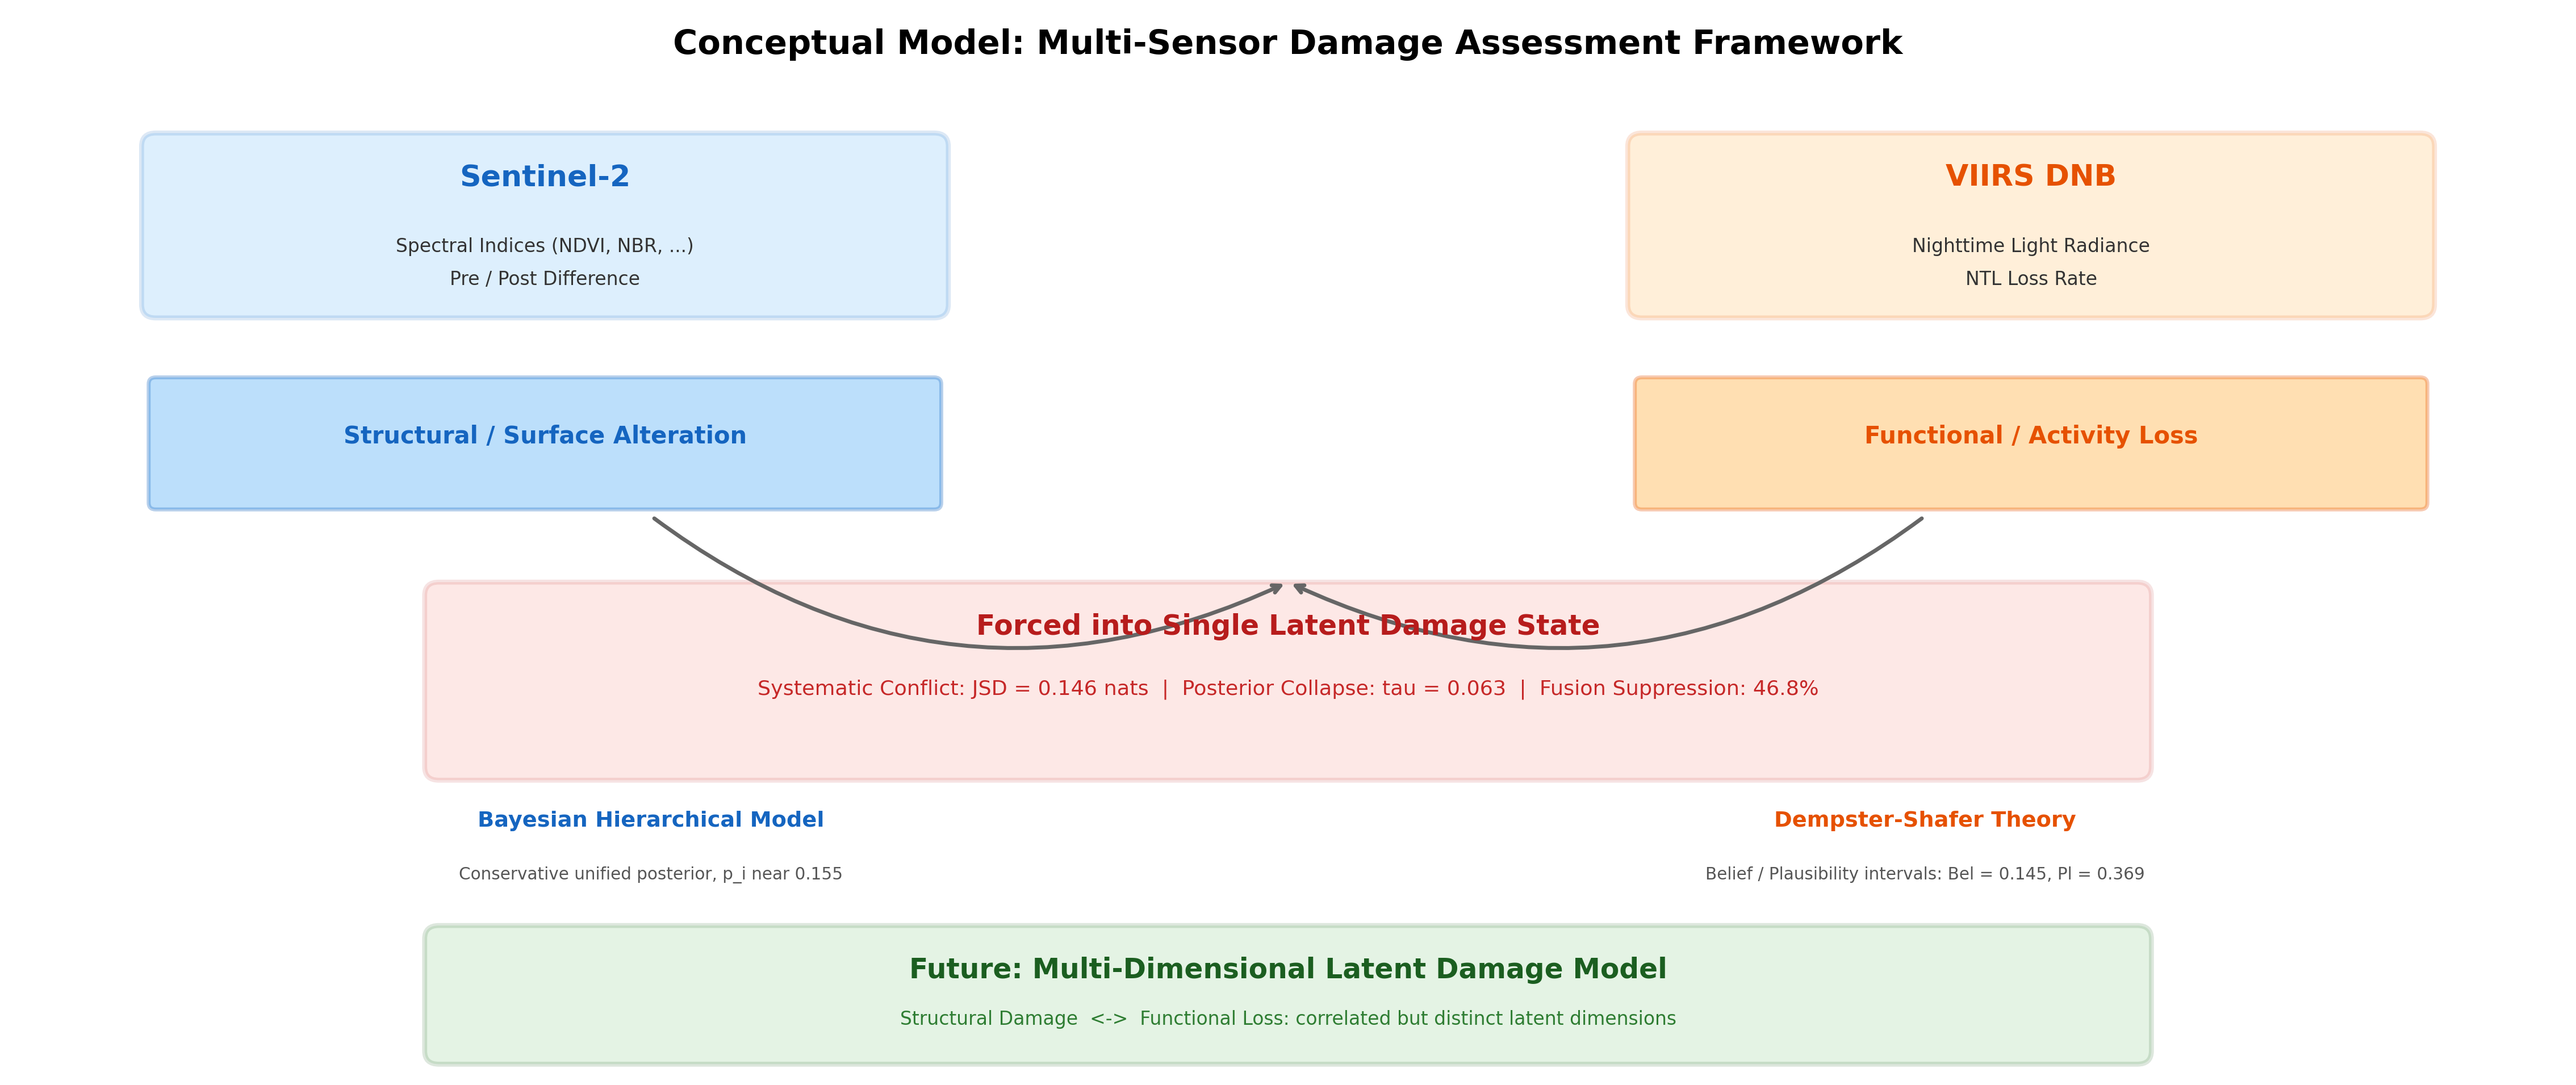
\includegraphics[width=0.95\textwidth]{figures/fig8_conceptual_model_v4.png}
\caption{\textbf{Conceptual model: from single latent state to
multi-dimensional damage assessment.} S2 captures structural/surface
alteration; VIIRS captures functional/activity loss. Forcing both into a
single latent state produces systematic conflict (JSD~$=0.146$ nats),
posterior collapse ($\tau=0.063$), and fusion suppression ($46.8\%$).
The Bayesian model yields a conservative unified posterior; D-S preserves
uncertainty intervals. Future work should model structural and functional
damage as correlated but distinct latent dimensions.}
\label{fig:concept}
\end{center}
\end{figure}

The contrast between Bayesian and D-S paradigms clarifies the trade-off
(Figure~\ref{fig:concept}). The Bayesian model provides a coherent
posterior but sacrifices spatial discrimination when evidence conflicts.
D-S preserves uncertainty through wider intervals but may over-weight
strong single-sensor evidence in the absence of hierarchical
regularization. Neither approach is universally superior; they serve
complementary roles. A natural extension is a multi-dimensional latent
damage model with correlated structural and functional damage states, where
each sensor primarily informs its corresponding dimension and a correlation
structure allows information sharing.

% =====================================================================
\section{Limitations}\label{sec:limitations}

\begin{enumerate}
  \item \textbf{UNOSAT is an external reference, not absolute ground truth.}
    It captures visually identifiable building damage but may miss
    functional damage, sub-detection-threshold structural alteration, or
    damage types outside its classification scheme.
  \item \textbf{Single-sensor MCMC diagnostics were weaker than the joint
    model.} The S2-only (263 divergences, $\hat{R}_{\max}=1.21$) and
    VIIRS-only (122 divergences, $\hat{R}_{\max}=1.35$) models showed
    elevated sampling issues; their posterior ranges should be interpreted
    as diagnostic comparisons.
  \item \textbf{Results are conditional on the 500~m grid scale.} Different
    spatial resolutions would yield different conflict and information gain
    estimates.
  \item \textbf{Temporal mismatch.} The S2 and VIIRS pre/post pairs capture
    slightly different time windows.
  \item \textbf{The current S2 index is one of many possible formulations.}
    Alternative spectral indices or texture features could produce
    different alignment with UNOSAT.
  \item \textbf{VIIRS NTL loss conflates multiple processes.} Reduced NTL
    can reflect building destruction, power grid damage, population
    displacement, or deliberate blackouts.
  \item \textbf{Single latent state model oversimplifies damage.}
    Structural damage and functional loss are distinct phenomena.
\end{enumerate}

% =====================================================================
\section{Conclusion}\label{sec:conclusion}

This study examined the fusion of Sentinel-2 spectral indices and VIIRS
nighttime light loss for damage assessment in Mariupol through three
complementary frameworks. Our findings form a coherent evidence chain
(Figure~\ref{fig:workflow}):

\textbf{A.} S2 and VIIRS provide non-equivalent damage signals ($r=-0.33$),
capturing structural surface alteration and functional activity loss
respectively (Figure~\ref{fig:disagree}).

\textbf{B.} Under this validation setting, VIIRS shows stronger agreement
with UNOSAT reference labels (AUC~$=0.829$) than the current S2-derived
index (AUC~$=0.332$). All fusion scores perform below VIIRS alone
(Figure~\ref{fig:unosat}).

\textbf{C1.} The Bayesian hierarchical model produces a near-uniform
posterior ($p_i \in [0.151, 0.157]$, $\tau=0.063$). Each sensor alone
retains spatial structure; collapse occurs only under joint fusion
(Figure~\ref{fig:bayes}).

\textbf{C2.} KLD/JSD demonstrates that spatial information is not absent
but suppressed by conflicting evidence. Fusion suppression ratio~$=46.8\%$;
JSD~$>0.05$ nats across all grids (Figures~\ref{fig:kld_summary}
--\ref{fig:kld_maps}).

\textbf{C3.} Bayesian and D-S paradigms show $49.9\%$ genuine agreement,
$10.2\%$ uncertainty-compatible, and $28.1\%$ divergence, reflecting
different strategies for handling conflicting evidence
(Figure~\ref{fig:ds}).

\textbf{D.} Adding sensors does not automatically improve damage estimation
(Figure~\ref{fig:concept}). Multi-sensor fusion benefits inference only when
sensors measure compatible damage dimensions or when the model explicitly
accommodates multiple latent states. We recommend moving toward
multi-dimensional latent damage models that distinguish structural and
functional damage as correlated but distinct phenomena.

% =====================================================================
%\acks{This work was supported by...}

\bibliography{references}

% =====================================================================
\appendix

\section{PR Curves for UNOSAT Validation}\label{apd:pr}

\begin{figure}[htp]
\begin{center}
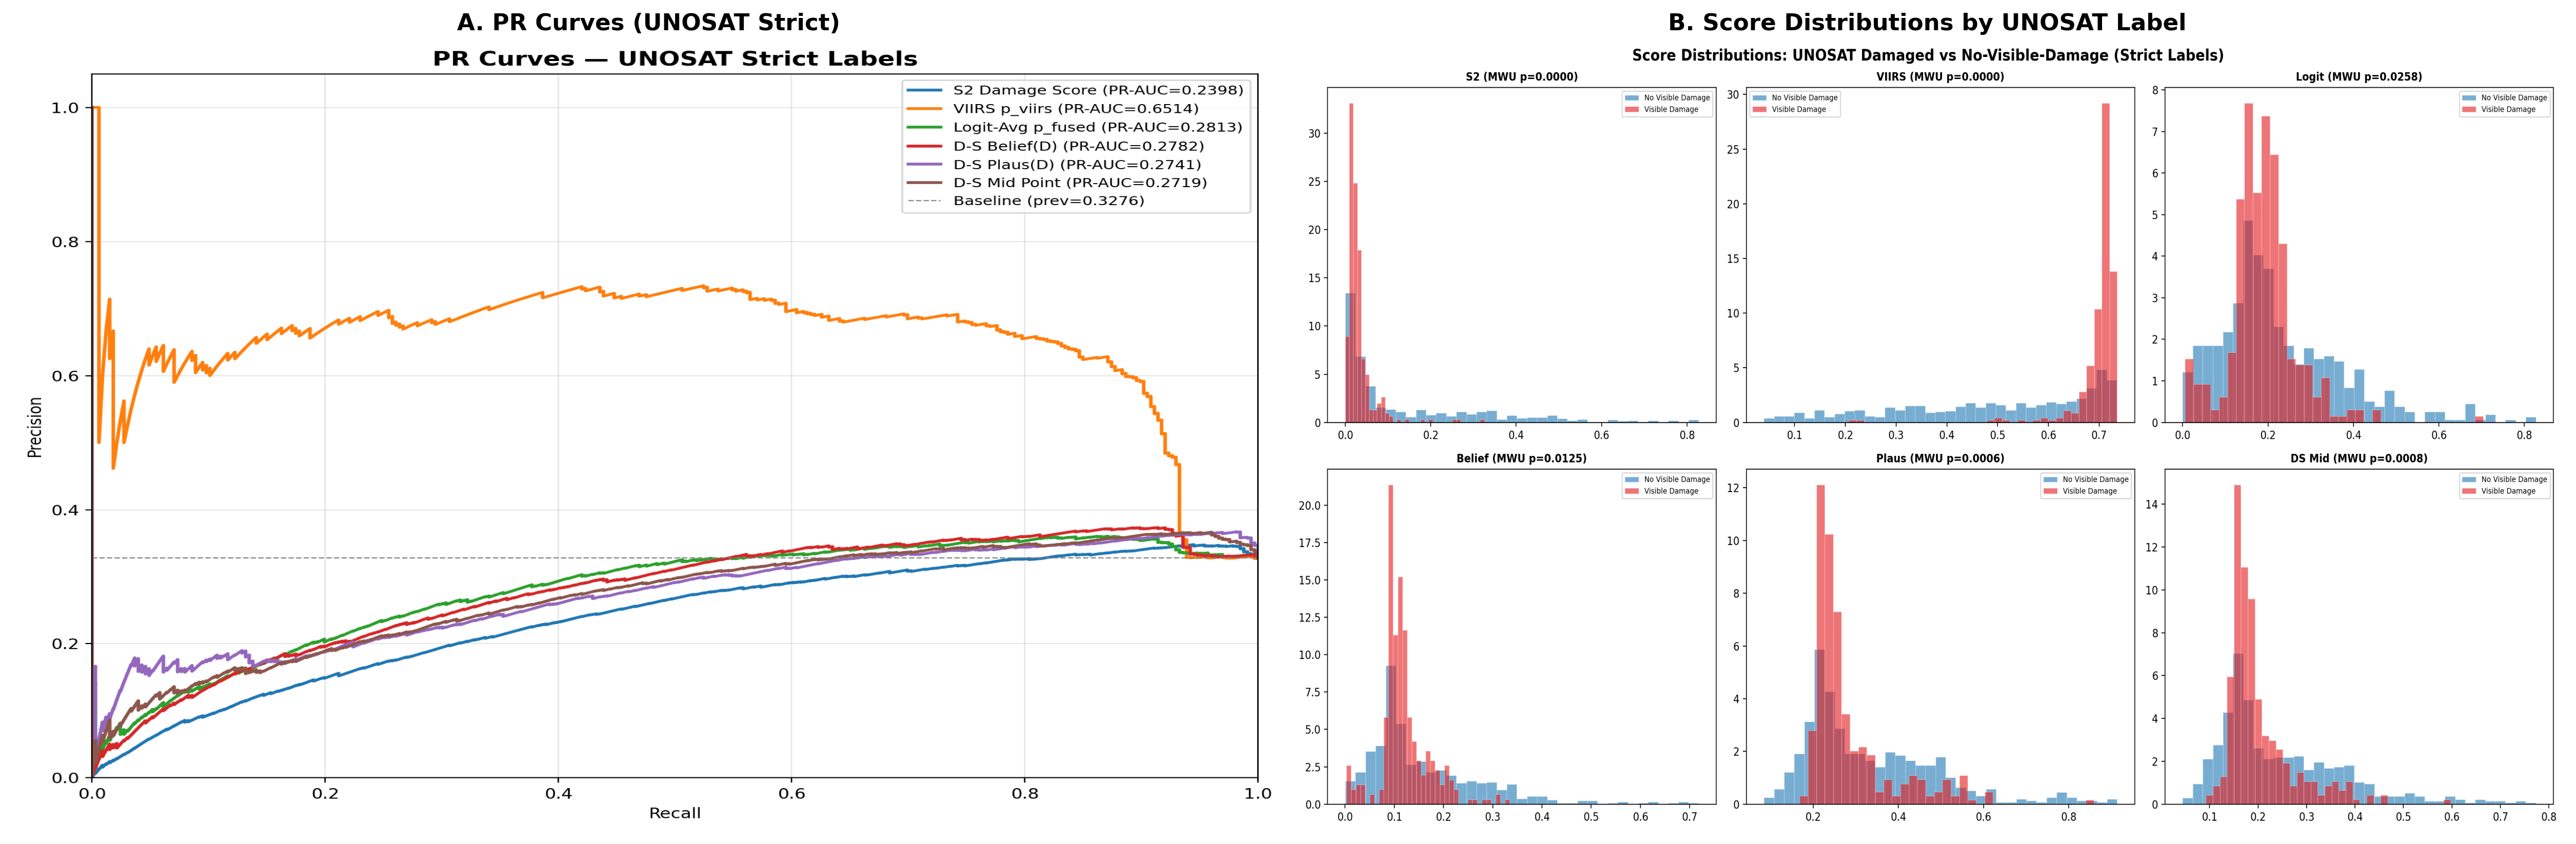
\includegraphics[width=0.85\textwidth]{figures/fig_appendix_pr_v4.png}
\caption{Precision-recall curves corresponding to Figure~\ref{fig:unosat}.}
\label{fig:pr_appendix}
\end{center}
\end{figure}

\section{Method Comparison}\label{apd:methods}

\begin{table}[htp]
\centering
\caption{Method comparison and interpretation.}
\label{tab:methods}
\begin{tabular}{@{}lp{4.5cm}p{5.5cm}@{}}
\toprule
\textbf{Method} & \textbf{What it provides} &
  \textbf{Key finding} \\
\midrule
S2 spectral index &
  Pixel-level surface change score &
  Detects surface alterations; weakly correlated with UNOSAT (AUC~$=0.33$) \\
VIIRS NTL-loss index &
  Grid-level functional loss score &
  Shows stronger agreement with UNOSAT (AUC~$=0.83$); may conflate
  structural and functional loss \\
UNOSAT validation &
  External reference (visual interpretation) &
  Structured benchmark; imperfect visual-only product \\
Bayesian hierarchical model &
  Unified posterior $p_i$ with 95\% CI &
  Reveals S2-VIIRS irreconcilability under single latent state \\
KLD/JSD analysis &
  Quantitative information and conflict per grid &
  Fusion suppression $46.8\%$; JSD $>0.05$ everywhere \\
D-S evidence theory &
  Belief/Plausibility interval &
  Preserves uncertainty (Bel~$=0.145$, Pl~$=0.369$) \\
Bayesian vs.\ D-S &
  Grid-level paradigm comparison &
  $49.9\%$ genuine agreement; $28.1\%$ divergent \\
\bottomrule
\end{tabular}
\end{table}

\section{JSD vs Divergence Scatter}\label{apd:scatter}

\begin{figure}[htp]
\begin{center}
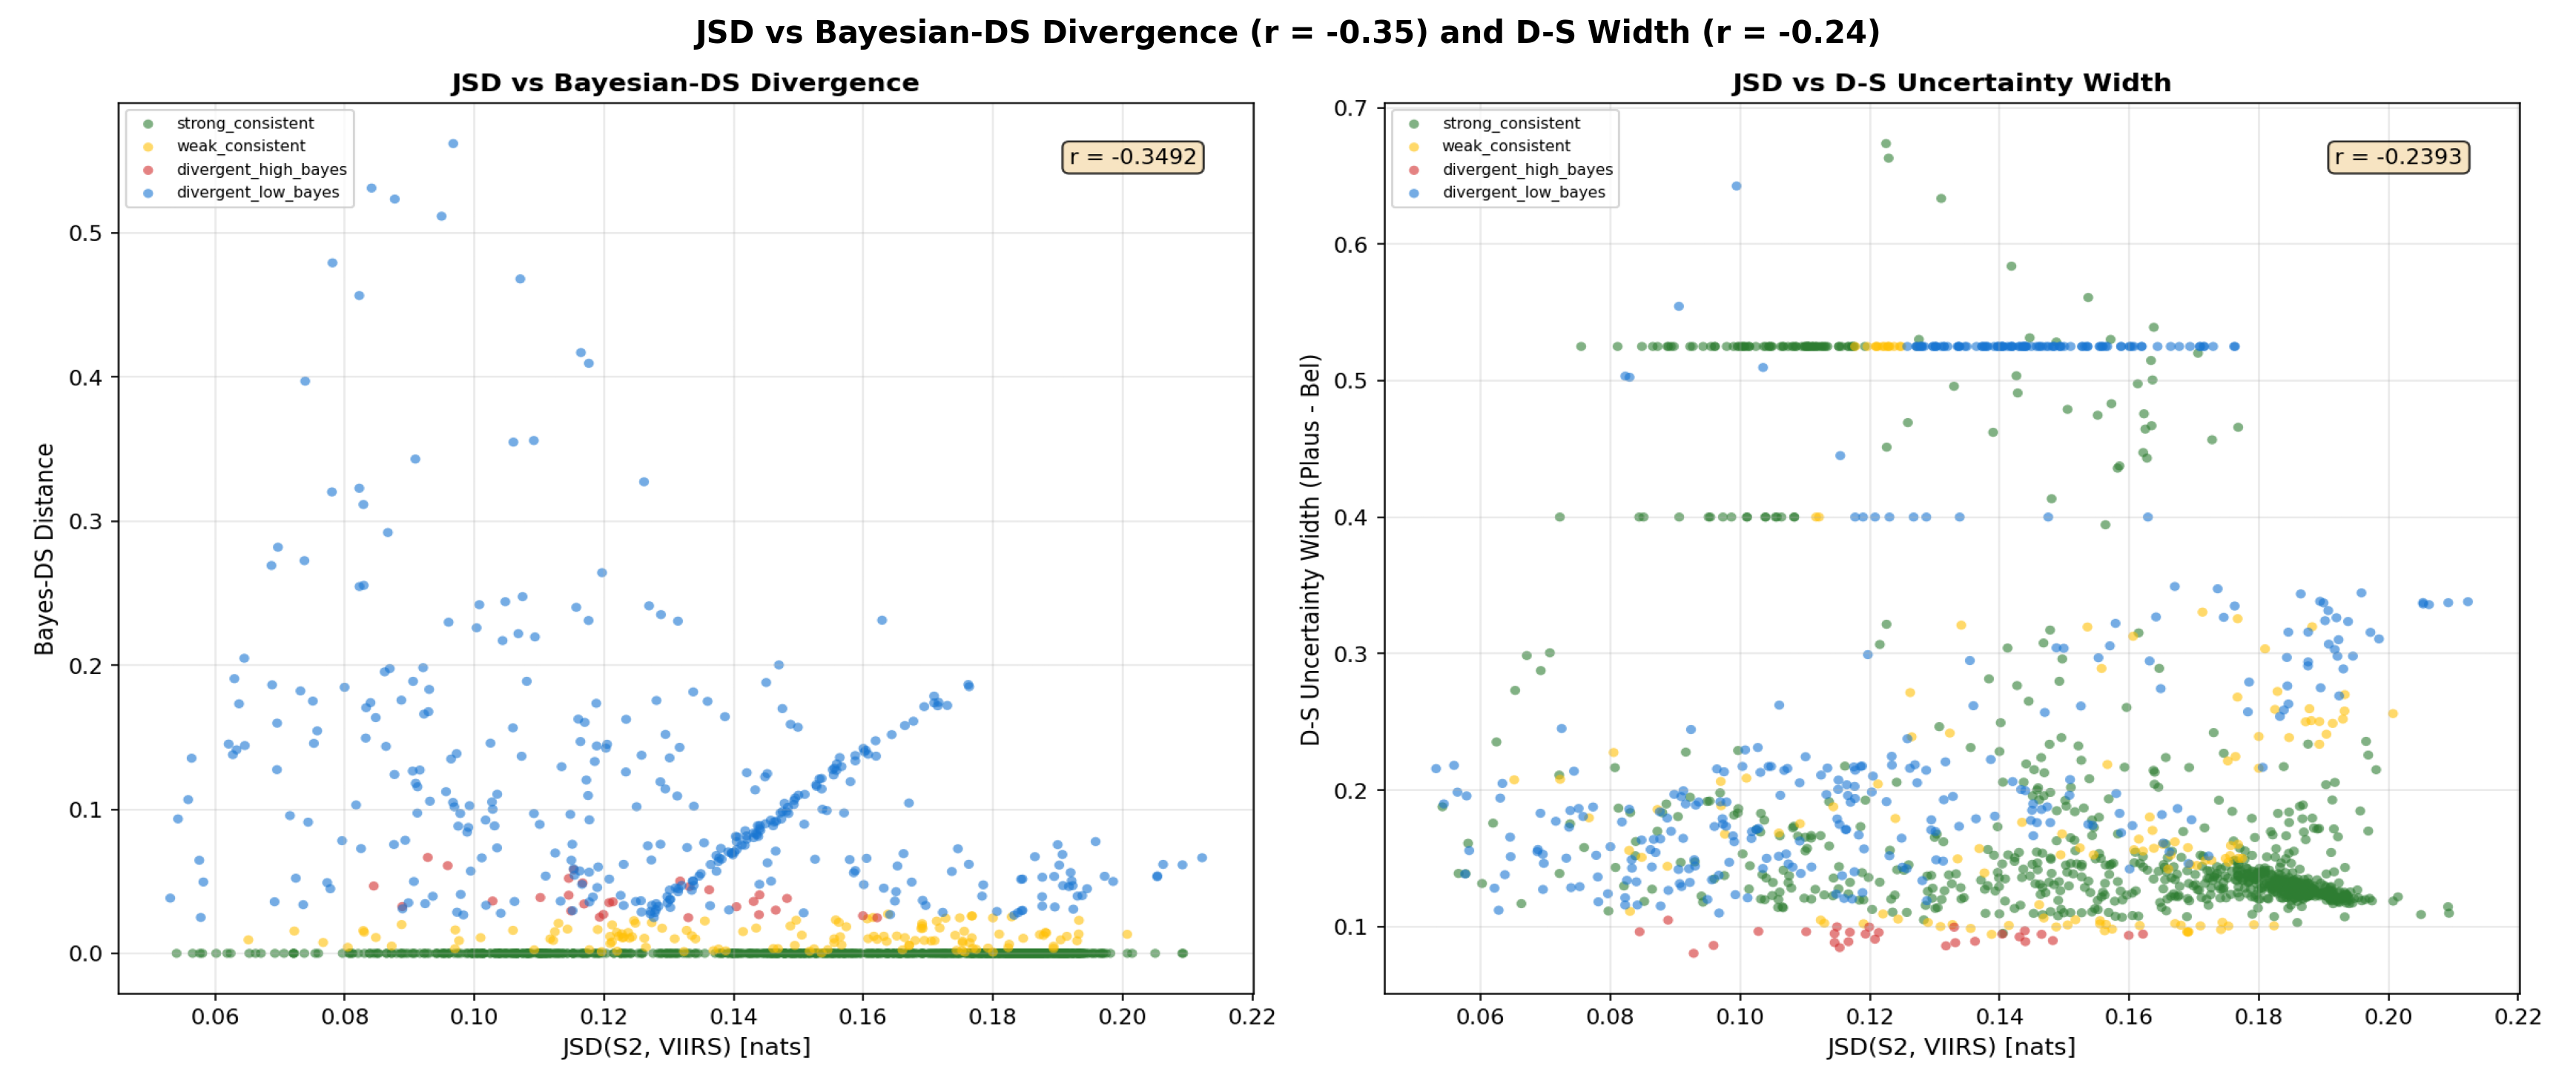
\includegraphics[width=0.85\textwidth]{figures/fig_appendix_scatter_v4.png}
\caption{JSD vs.\ Bayesian-DS divergence ($r=-0.35$, left) and JSD vs.\
D-S uncertainty width ($r=-0.24$, right).}
\label{fig:scatter_appendix}
\end{center}
\end{figure}

\end{document}
